\documentclass{beamer}
\usepackage{pgf,pgfarrows,pgfnodes,pgfautomata,pgfheaps}
\usepackage{amsmath,amssymb}
\usepackage{graphics}
%\usepackage{multimedia}
%\usepackage{movie15}
\usepackage{beamerthemesplit} 
\usepackage{beamerthemeshadow}

%%%%%%%%%%%%%%%%%%%%%%%%%%%%%%%%%%%%%%%%%%%%%%%%%%%%%%
\usepackage{xeCJK}
%\usepackage{fontspec}
\setCJKmainfont[BoldFont=simhei.ttf]{simsun.ttf}
\setCJKsansfont{simhei.ttf}
\setCJKmonofont{simfang.ttf}
%%%%%%%%%%%%%%%%%%%%%%%%%%%%%%%%%%%%%%%%%%%%%%%%%%%%%%
\graphicspath{{figures/}}
\renewcommand{\raggedright}{\leftskip=0pt \rightskip=0pt plus 0cm}
\raggedright

\begin{document}
%% ����Ĵ�����������Logoͼ��
%\pgfdeclaremask{logomask}{pku-tower-mask}
%\pgfdeclareimage[mask=logomask,height=1.5cm]{logo}{pku-tower}


\pgfdeclaremask{beidamask}{./picture/CAS-blue.pdf}
\pgfdeclareimage[mask=beidamask,height=0.25cm]{beida}{./figures/CAS-blue.pdf}

%\pgfdeclaremask{titlemask}{pku-lake2-mask}
%\pgfdeclareimage[mask=titlemask,height=2.5cm]{title}{pku-lake2}

%\logo{\vbox{\hbox{\hfill\pgfuseimage{logo}}}} %����logoͼ��

%% ����һЩ��ѡ��ģ�壬����������ͼ�ꡢ��������ҳ�ŵȣ��޸�Ҫ����
\beamertemplateshadingbackground{red!10}{structure!10}
%\beamertemplatesolidbackgroundcolor{white!90!blue}
\beamertemplatetransparentcovereddynamic
\beamertemplateballitem
\beamertemplatenumberedballsectiontoc
%\beamertemplatelargetitlepage
\beamertemplateboldpartpage

\makeatletter
\usefoottemplate{ %���¶���ҳ�ţ��������ߣ���λ����λͼ�꣬���ĵ�����
  \vbox{\tiny%
    \hbox{%
      \setbox\beamer@linebox=\hbox to\paperwidth{%
        \hbox to.5\paperwidth{\hfill\tiny\color{white}\textbf{\insertshortauthor\quad\insertshortinstitute}\hskip.1cm\lower 0.35em\hbox{\pgfuseimage{beida}}\hskip.3cm}%
        \hbox to.5\paperwidth{\hskip.3cm\tiny\color{white}\textbf{\insertshorttitle}\hfill}\hfill}%
      \ht\beamer@linebox=2.625ex%
      \dp\beamer@linebox=0pt%
      \setbox\beamer@linebox=\vbox{\box\beamer@linebox\vskip1.125ex}%
      \color{structure}\hskip-\Gm@lmargin\vrule width.5\paperwidth
      height\ht\beamer@linebox\color{structure!70}\vrule width.5\paperwidth
      height\ht\beamer@linebox\hskip-\paperwidth%
      \hbox{\box\beamer@linebox\hfill}\hfill\hskip-\Gm@rmargin}
  }
}
\makeatother


\title{超声速流场显示实验答辩}
\subtitle{力学实验与技术原理}
\author[第一组]{指导教师:顾洪斌\\第一组:周吕文{~}娄开元{~}王祺{~~}姜智捷}
\institute[中国科学院研究生院]{中国科学院研究生院}
\date{2012年7月3日}
\frame[plain]{\titlepage} % 产生主题页,plain选项表示不显示页眉页脚等内容

\subject{Computer Tools, TeX, Slide}
\titlegraphic{\pgfuseimage{title}}
\AtBeginSection[]{ % 在每个Section前都会加入的Frame
  \frame<handout:0>{
    \frametitle{Outline}
    \tableofcontents[current,currentsubsection]
  }
}


\section{实验背景}

\frame{\frametitle{流场显示实验溯源及应用}
\begin{columns}
\begin{column}[c]{0.4\textwidth}
\begin{center}
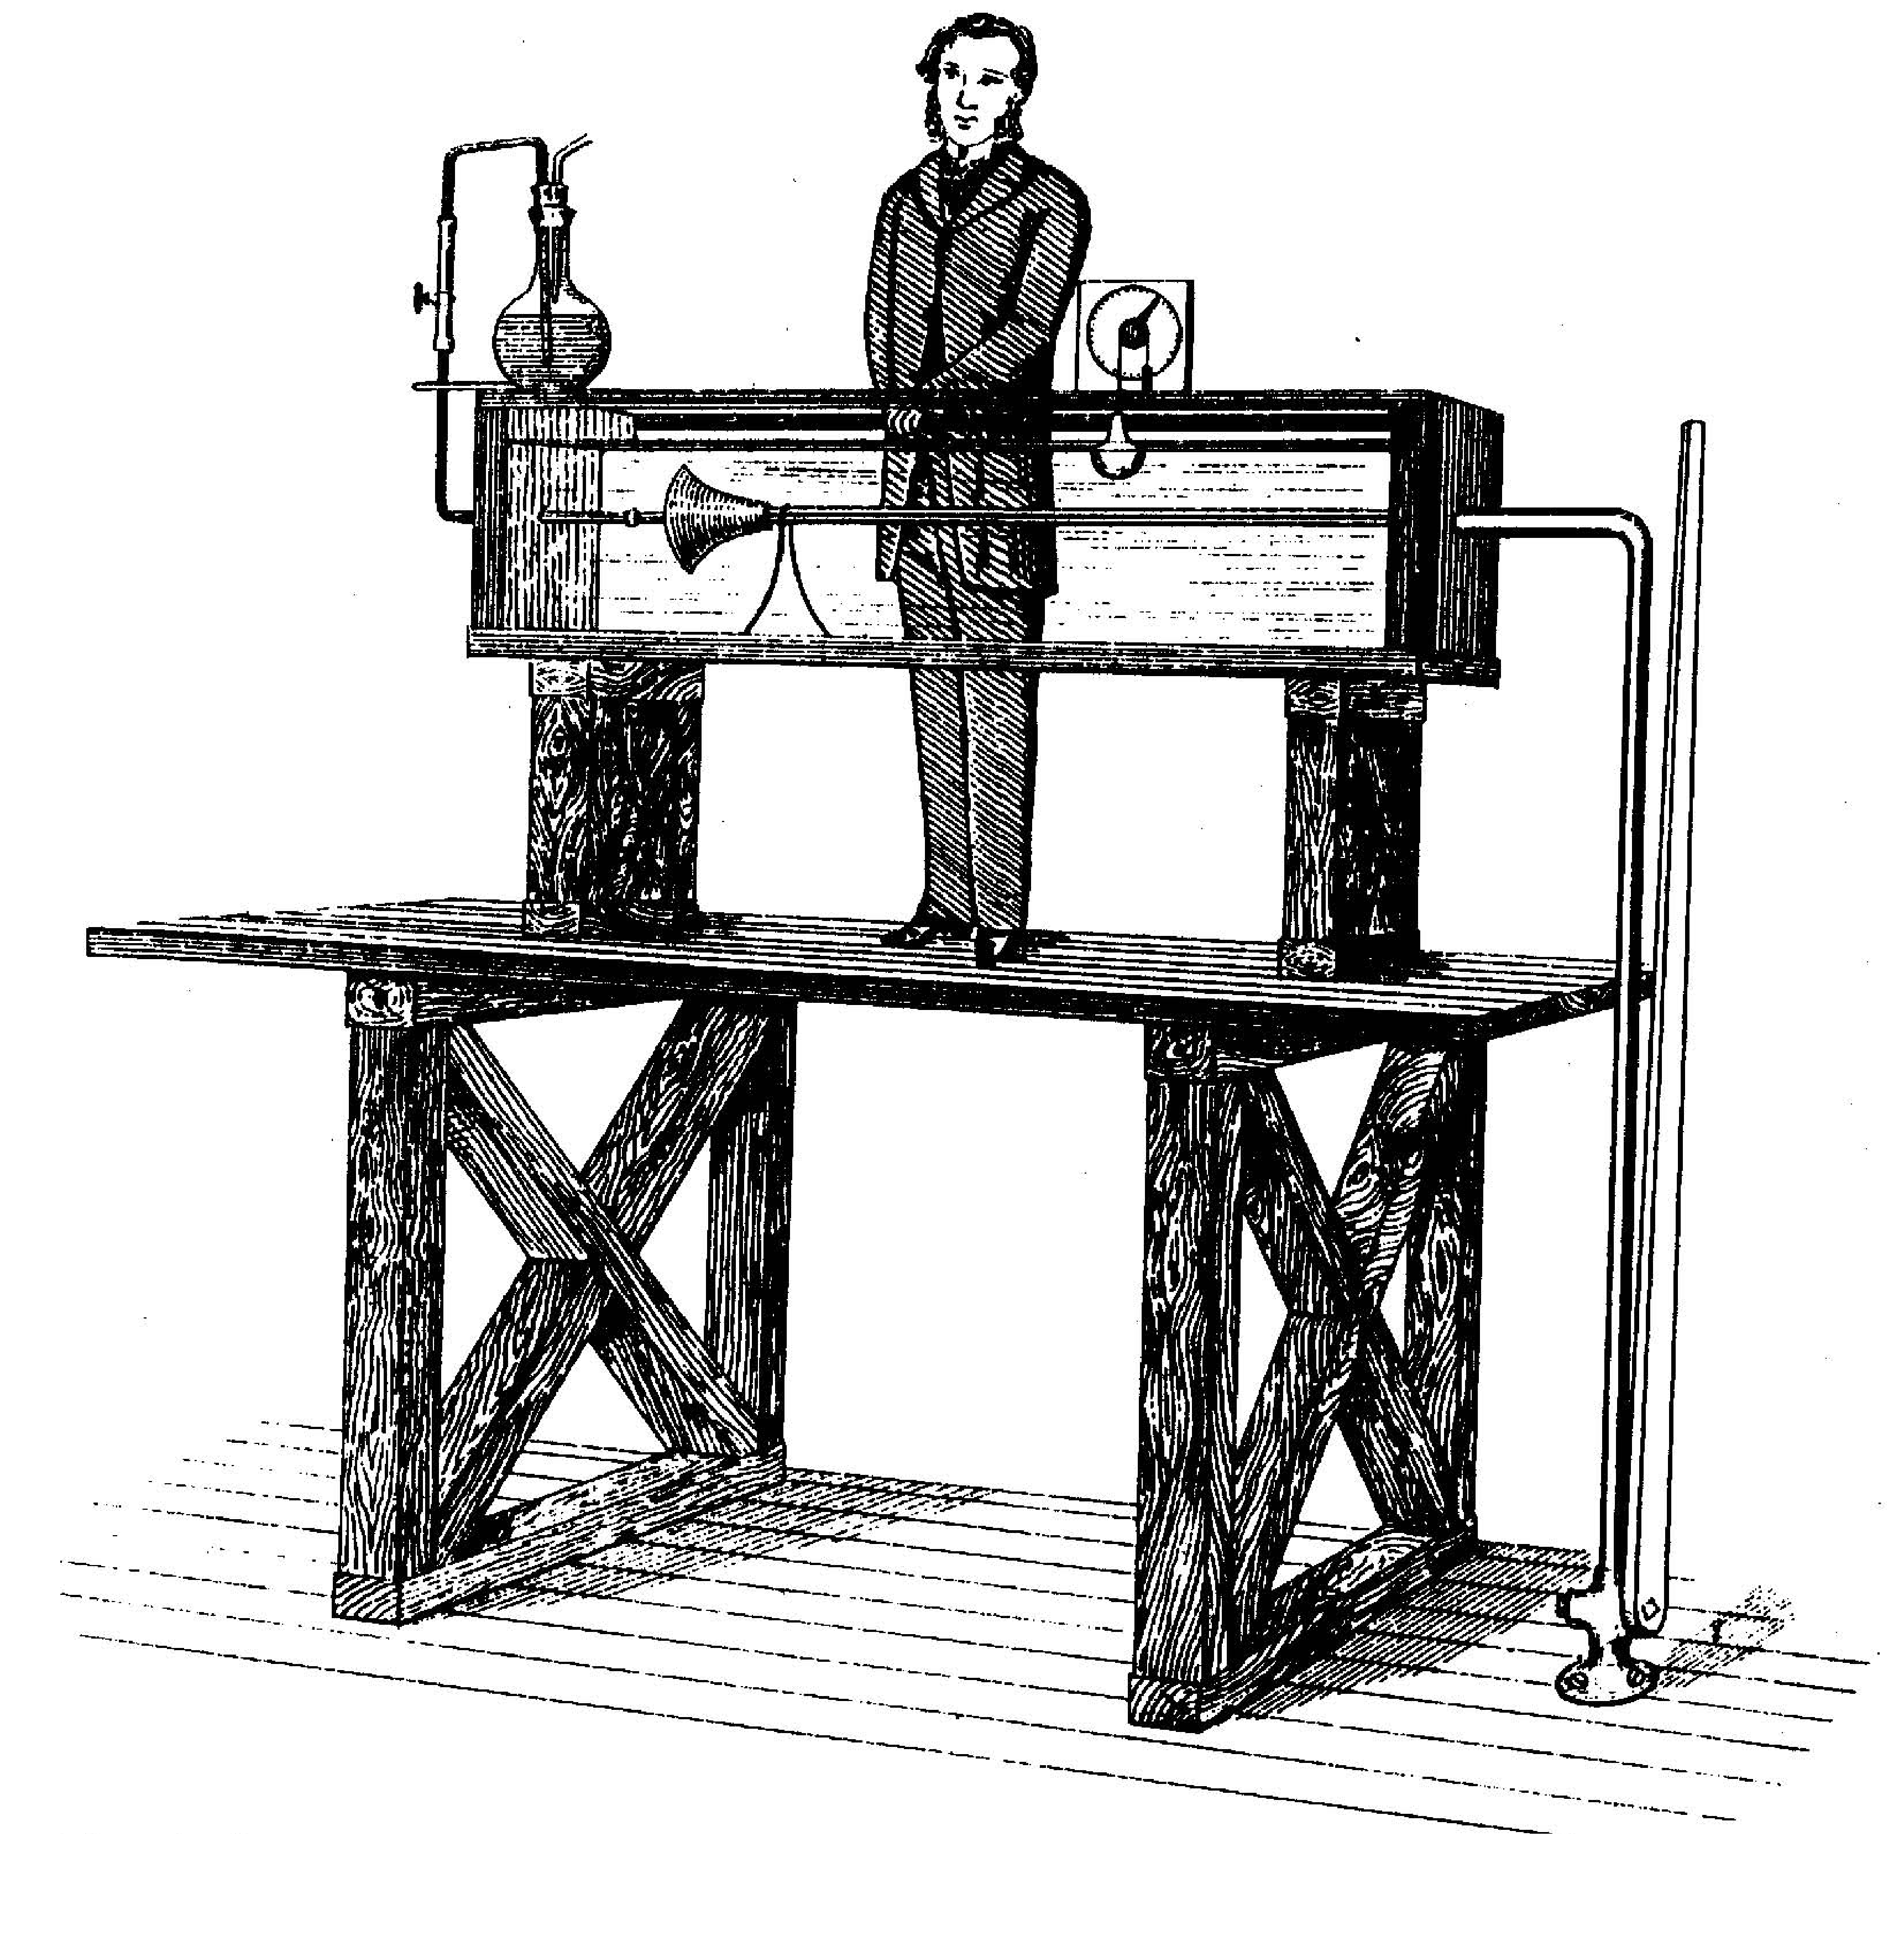
\includegraphics[width=1\textwidth]{Reynold.pdf}
\end{center}
\end{column}
\begin{column}[l]{0.6\textwidth}
\begin{itemize}
\item 流场显示实验可以追溯到1883年雷诺的流场显示实验.
\item 自雷诺实验后, 这门技术的原理性和技术性文献不断涌现, 形成了一门独特的实验技术科学.
\item 流场显示技术已被广泛应用于流体力学、空气动力学、爆炸力学、等离子体物理、燃烧学、传热学、核子物理等一系列领域中.
\end{itemize}
\end{column}
\end{columns}
}

\frame{\frametitle{常用流场显示技术}
常用流场显示技术有:
\begin{itemize}
\item \textbf{外加物质法}: 在透明无色的气流或水流中加入一些可见的粒子, 通过可见的外加粒子跟随流体微团的运动来使各种流动现象显示出来.(氢气泡, 染料溶液等)
\item \textbf{注入能量法}: 将能量加到流场中的部分流体上, 使它们的某些性质(如密度, 辐射能)与其它部分的流体区别开来, 以便用光学方法加以观察和记录. 加入能量的方式有电热丝加热, 电极放电, 激光聚焦, 电子束等.
\item \textbf{光学方法}: 利用流场的光学性质, 如气体的光学折射率是其密度的函数, 通过流场的折射率变化来显示某些流动现象, 通常用于高速流场中.
\end{itemize}
}


\section{实验原理}
\subsection{基本光学原理}
\frame{\frametitle{折射率与密度}
光在不同介质中的传播速度是不同的, 与介质的折射率$n$有关.
\[
n = \frac{c}{v} = 1 + \frac{c-v}{v} = 1 + \frac{\Delta\lambda}{\lambda}
\]

对于一定的介质, 其折射率是介质密度的函数, 当n接近为1时, 通常可以将上式近似表达为:
\[
\frac{n-1}{\rho} = K_{GD} {~}\textrm{或}{~} n=1+K_{GD}\rho
\]
上式称为Gladstone-Dale公式, 其中$K_{GD}$为常数, 是气体的一种特性, 称为比折射度. 一般情况下, 气体密度$\rho$与气体折射率$n$的关系可用上述Gladstone-Dale公式表示.
}

\frame{\frametitle{光线传输过程中的三个变量}
\begin{center}
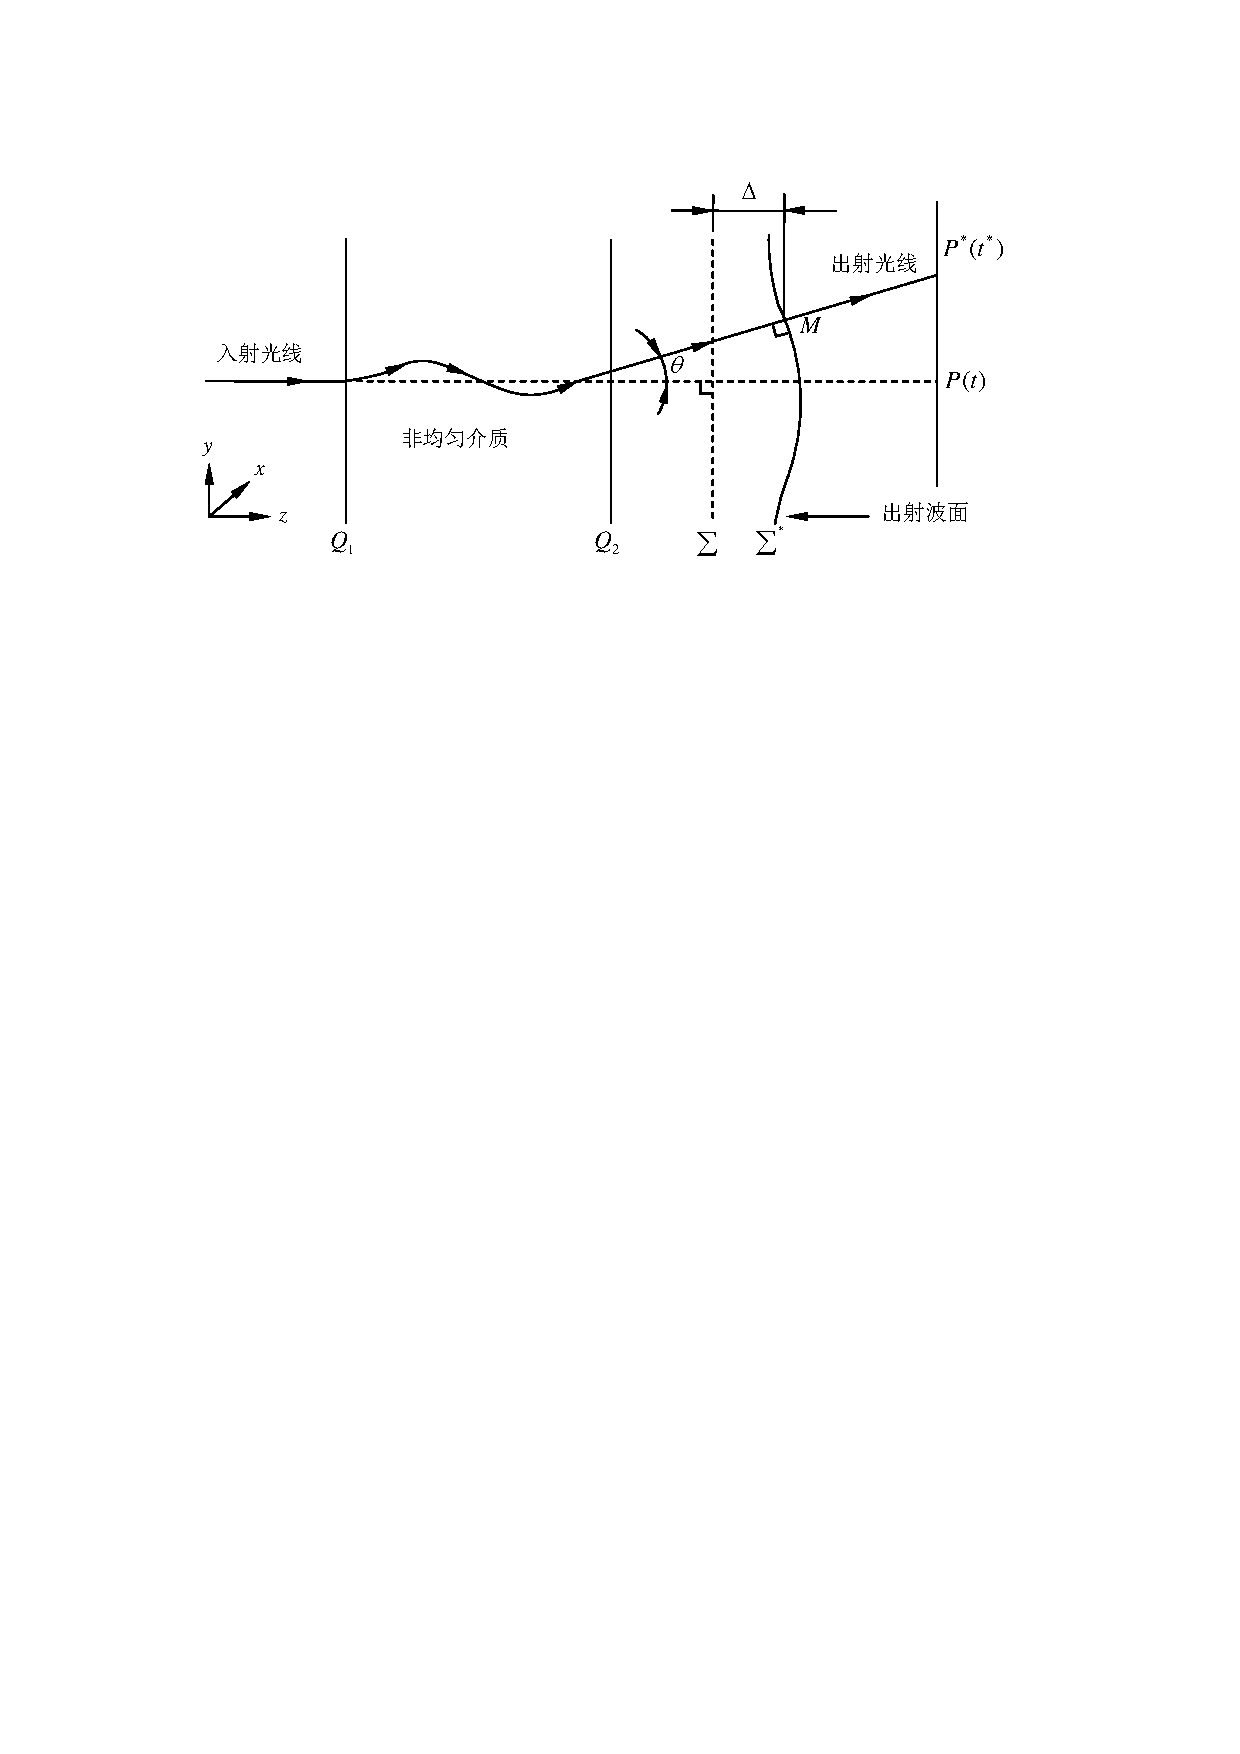
\includegraphics[width=0.9\textwidth]{optics.pdf}\\
\vspace{1em}

\textcolor{blue}{
\begin{tabular}{lll}
接收屏上的光线位移量($P^*P$) &  & $\partial^2\rho/\partial x^2$ \\
扰动与未扰动光线间的角偏移($\theta^*-\theta$) &   & $\partial\rho/\partial x$\\
光线的光程差引起的相位变化($\varphi^*-\varphi$) &  & $d\rho/dt$ \\
\end{tabular}
}
\end{center}
}

\subsection{阴影法}
\frame{\frametitle{阴影法}
\begin{columns}
\begin{column}[c]{0.5\textwidth}
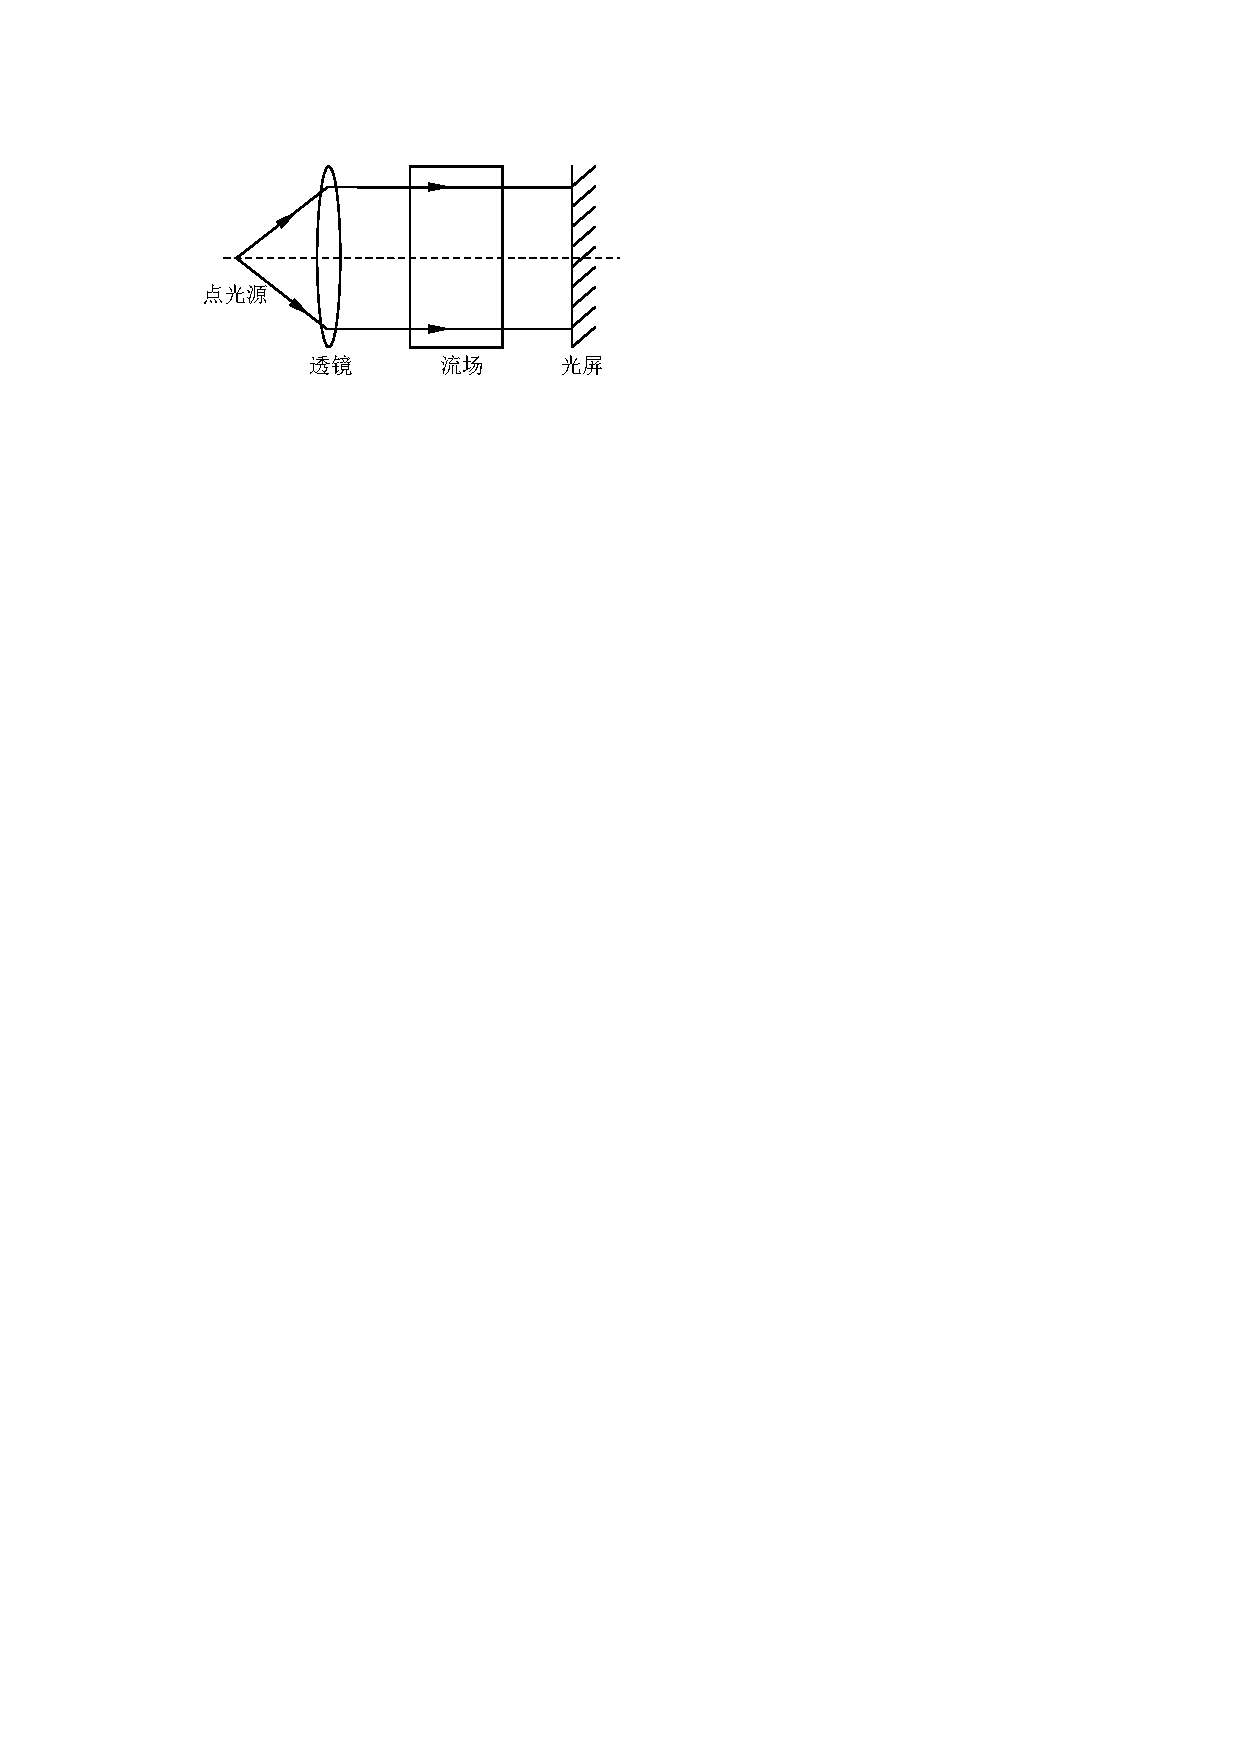
\includegraphics[width=0.9\textwidth]{shadow01.pdf}
\vspace{1em}

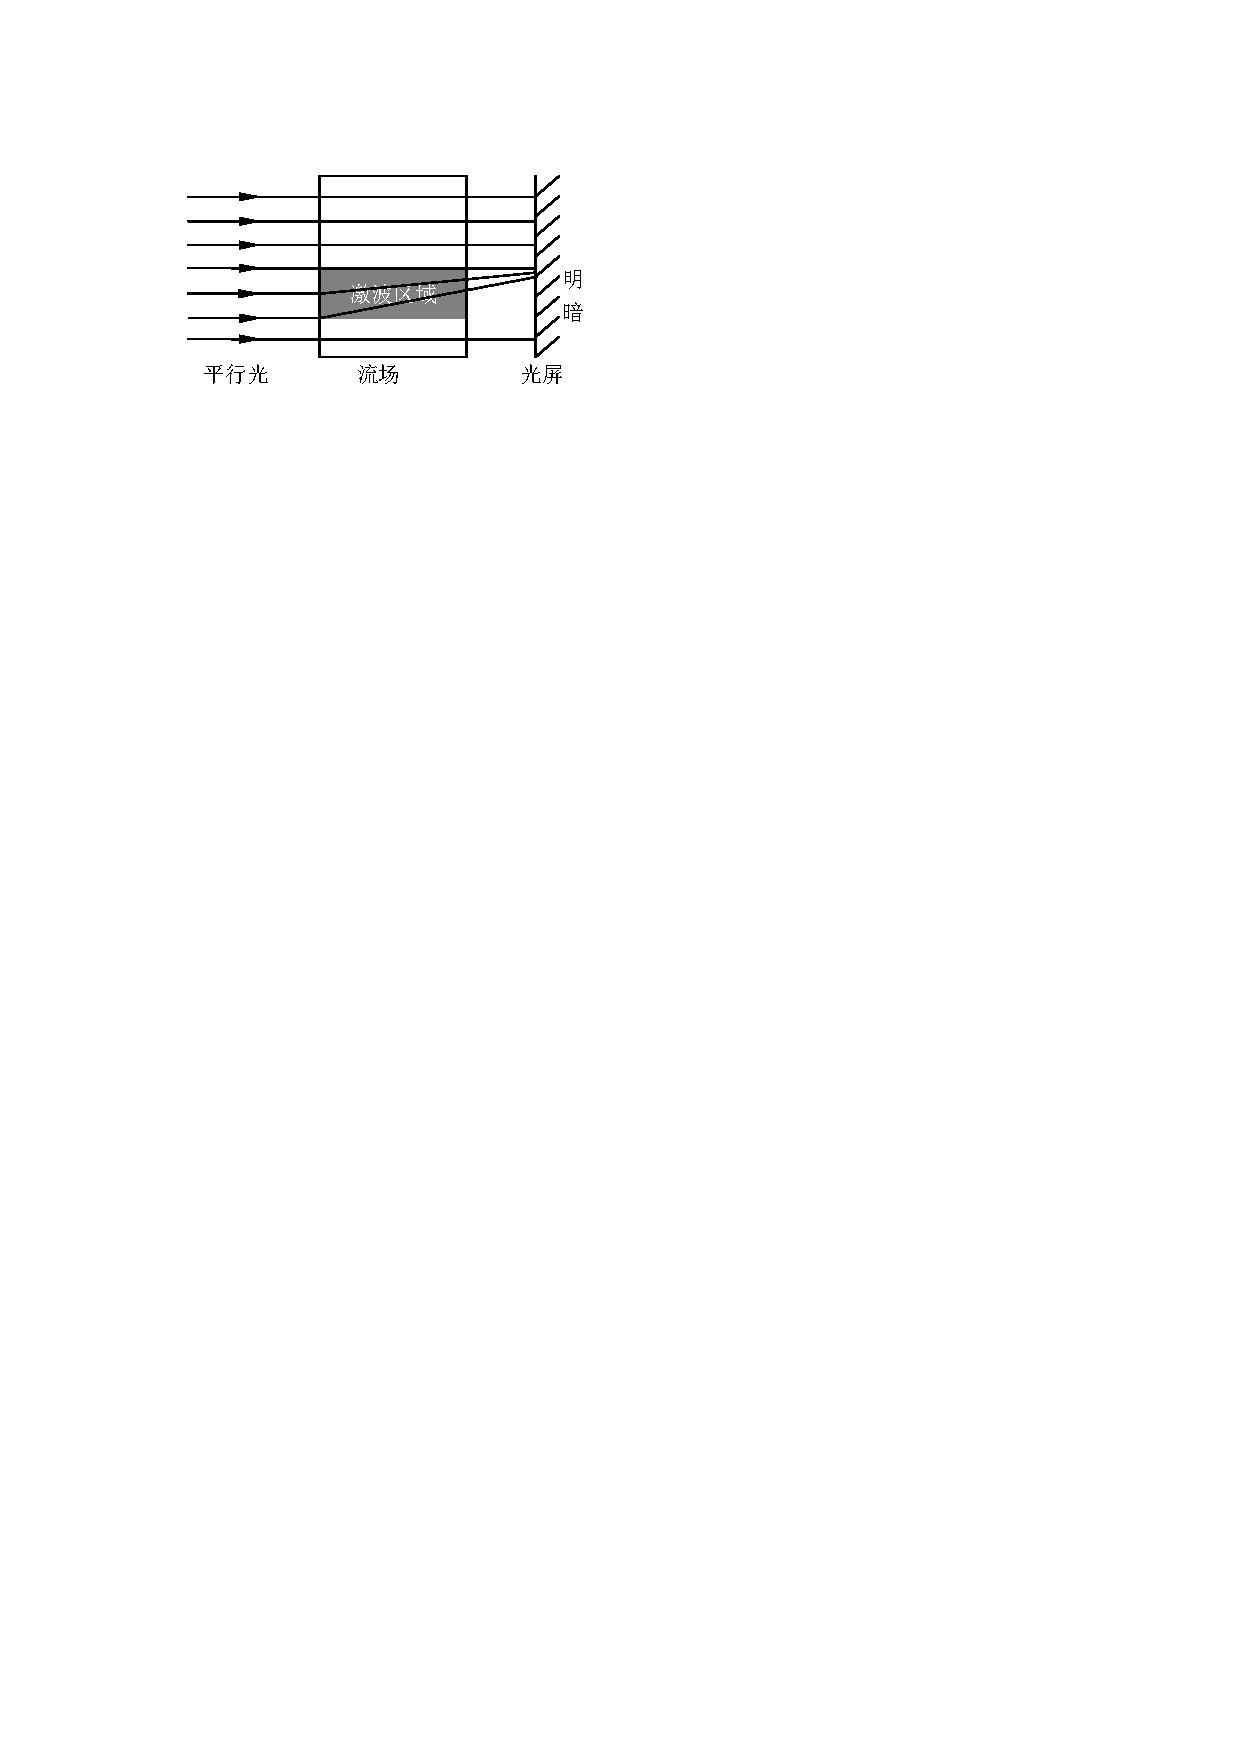
\includegraphics[width=0.91\textwidth]{shadow02.pdf}
\end{column}
\begin{column}[c]{0.5\textwidth}
\begin{itemize}
\item 流场中非激波区各点的折射率相同. 折射率的二阶导数$\partial^2n/\partial x^2=0$. 光线依然保持平行, 亮度不变.

\item 激波区存在很大的密度梯度. 在激波前锋部分,  折射率的二阶导数$\partial^2n/\partial x^2>0$, 光线散开, 屏幕上相应部分变暗.

\item 激波的后半部, 折射率的二阶导数$\partial^2n/\partial x^2<0$, 光线聚拢, 屏幕上相应部分变亮.
\end{itemize}
\end{column}
\end{columns}
}

\subsection{纹影法}
\frame{\frametitle{纹影法}
\begin{center}
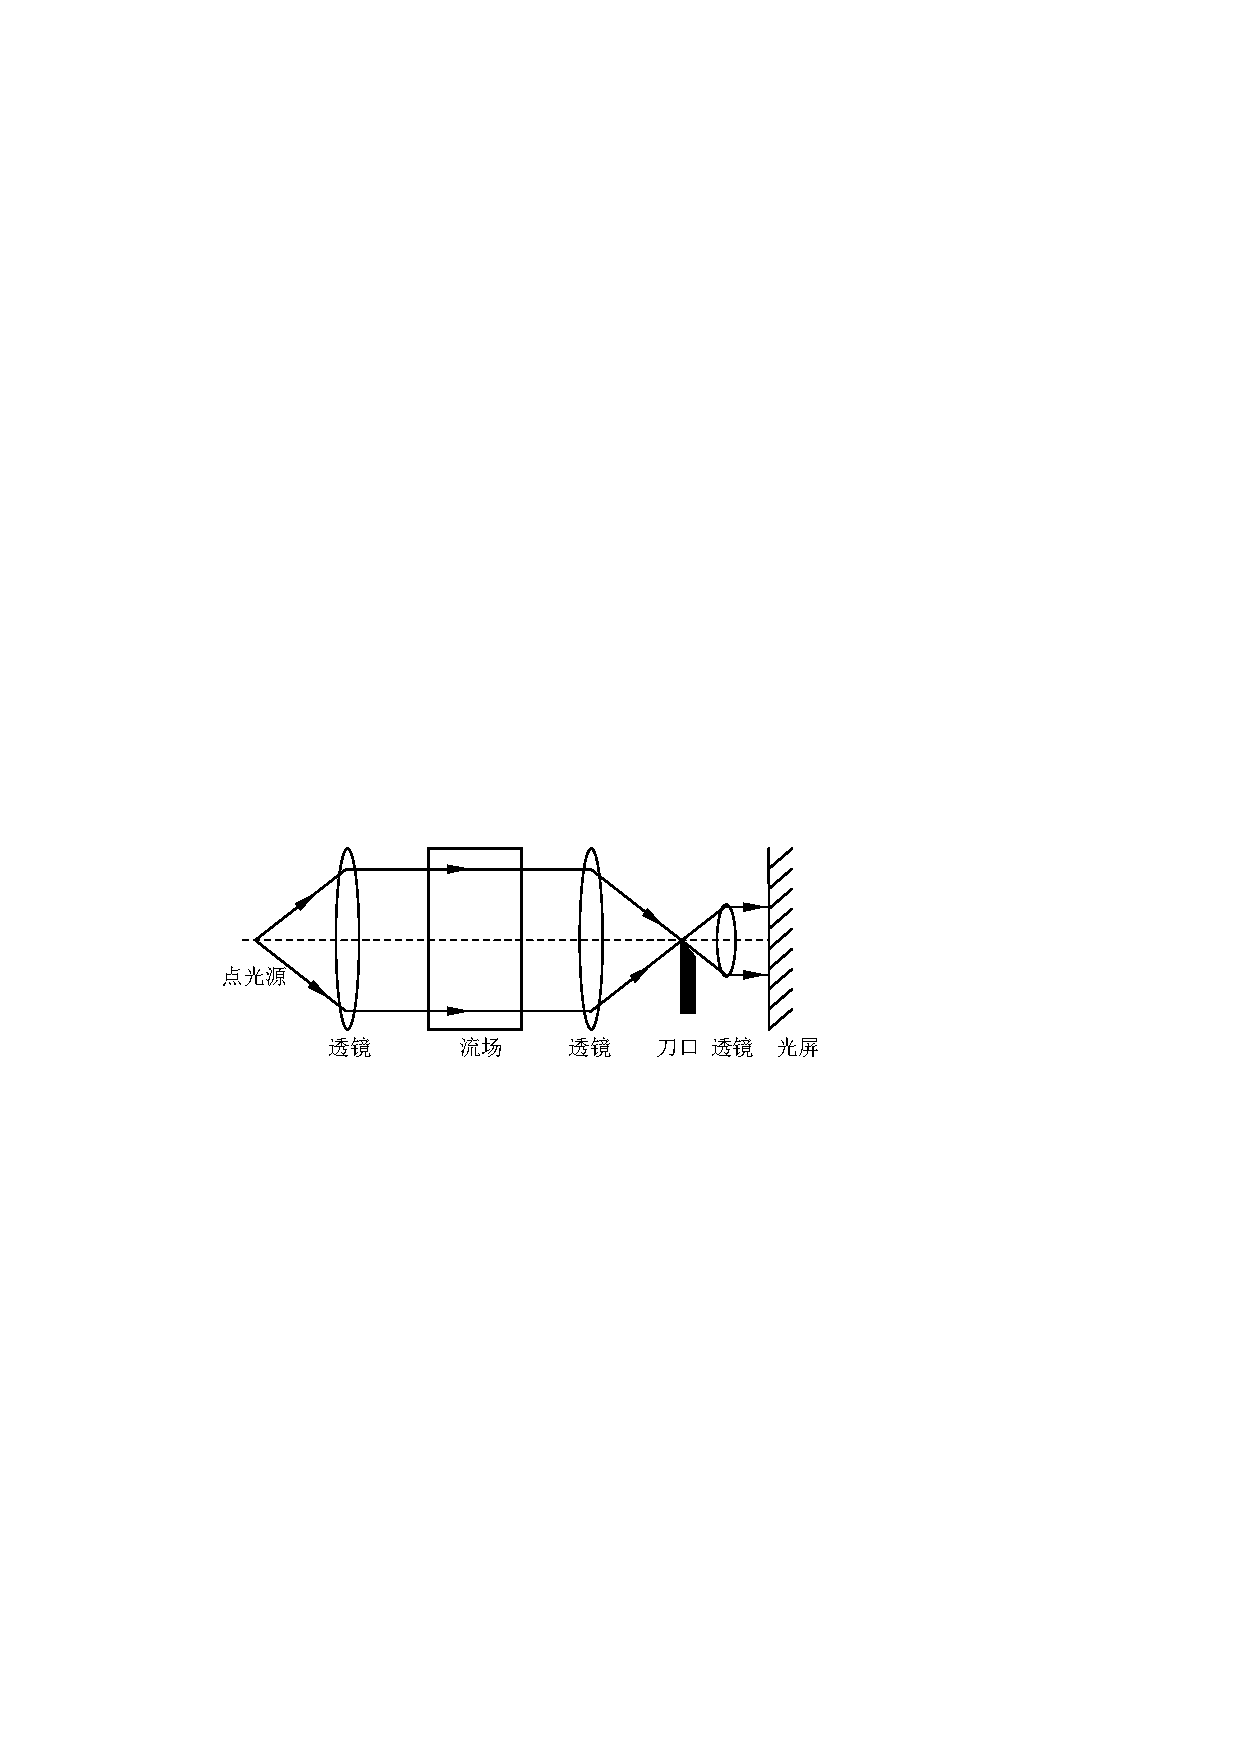
\includegraphics[width=0.8\textwidth]{schlieren01.pdf}
\end{center}

\begin{itemize}
\item 气流不均匀, 光线就会发生偏折. 向上折射$\Delta\theta$角的光线就会越过刀口光阑射到屏幕上, 幕上某些点由于额外多照射一些光线, 就比其他点亮一些.
\item 向下折射$\Delta\theta$的这部分光线就受到刀口光阑的阻挡, 幕上某些点就会比原来暗一些.
\item 屏幕上各点的阴暗程度取决于光线的偏折角$\Delta\theta$,对应于$\partial\rho/\partial x$.
\end{itemize}
}

\section{实验方案}
\subsection{阴影法}
\frame{\frametitle{阴影法}
\begin{center}
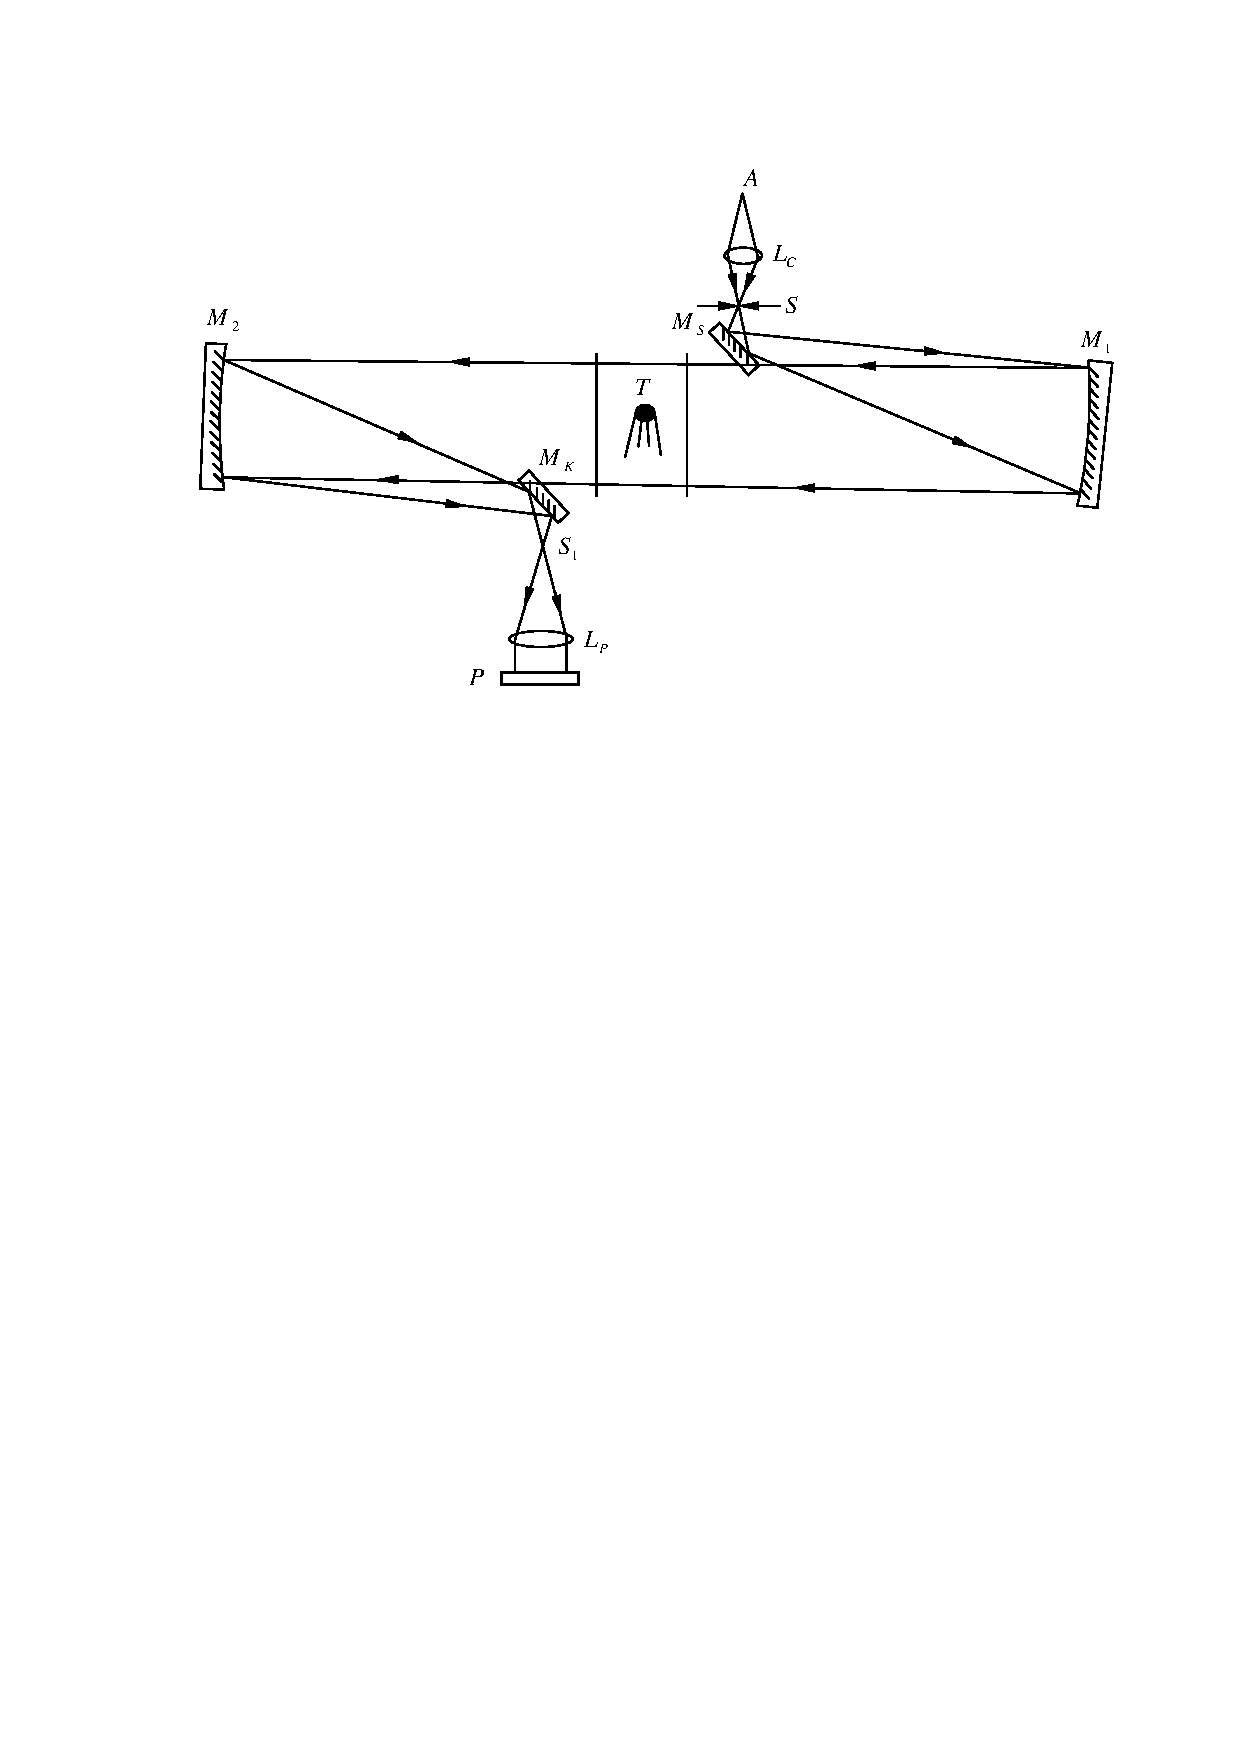
\includegraphics[width=0.85\textwidth]{shadow.pdf}\\
\textcolor{blue}{平行光聚焦阴影系统}
\end{center}
}

\subsection{纹影法}
\frame{\frametitle{纹影法}
\begin{center}
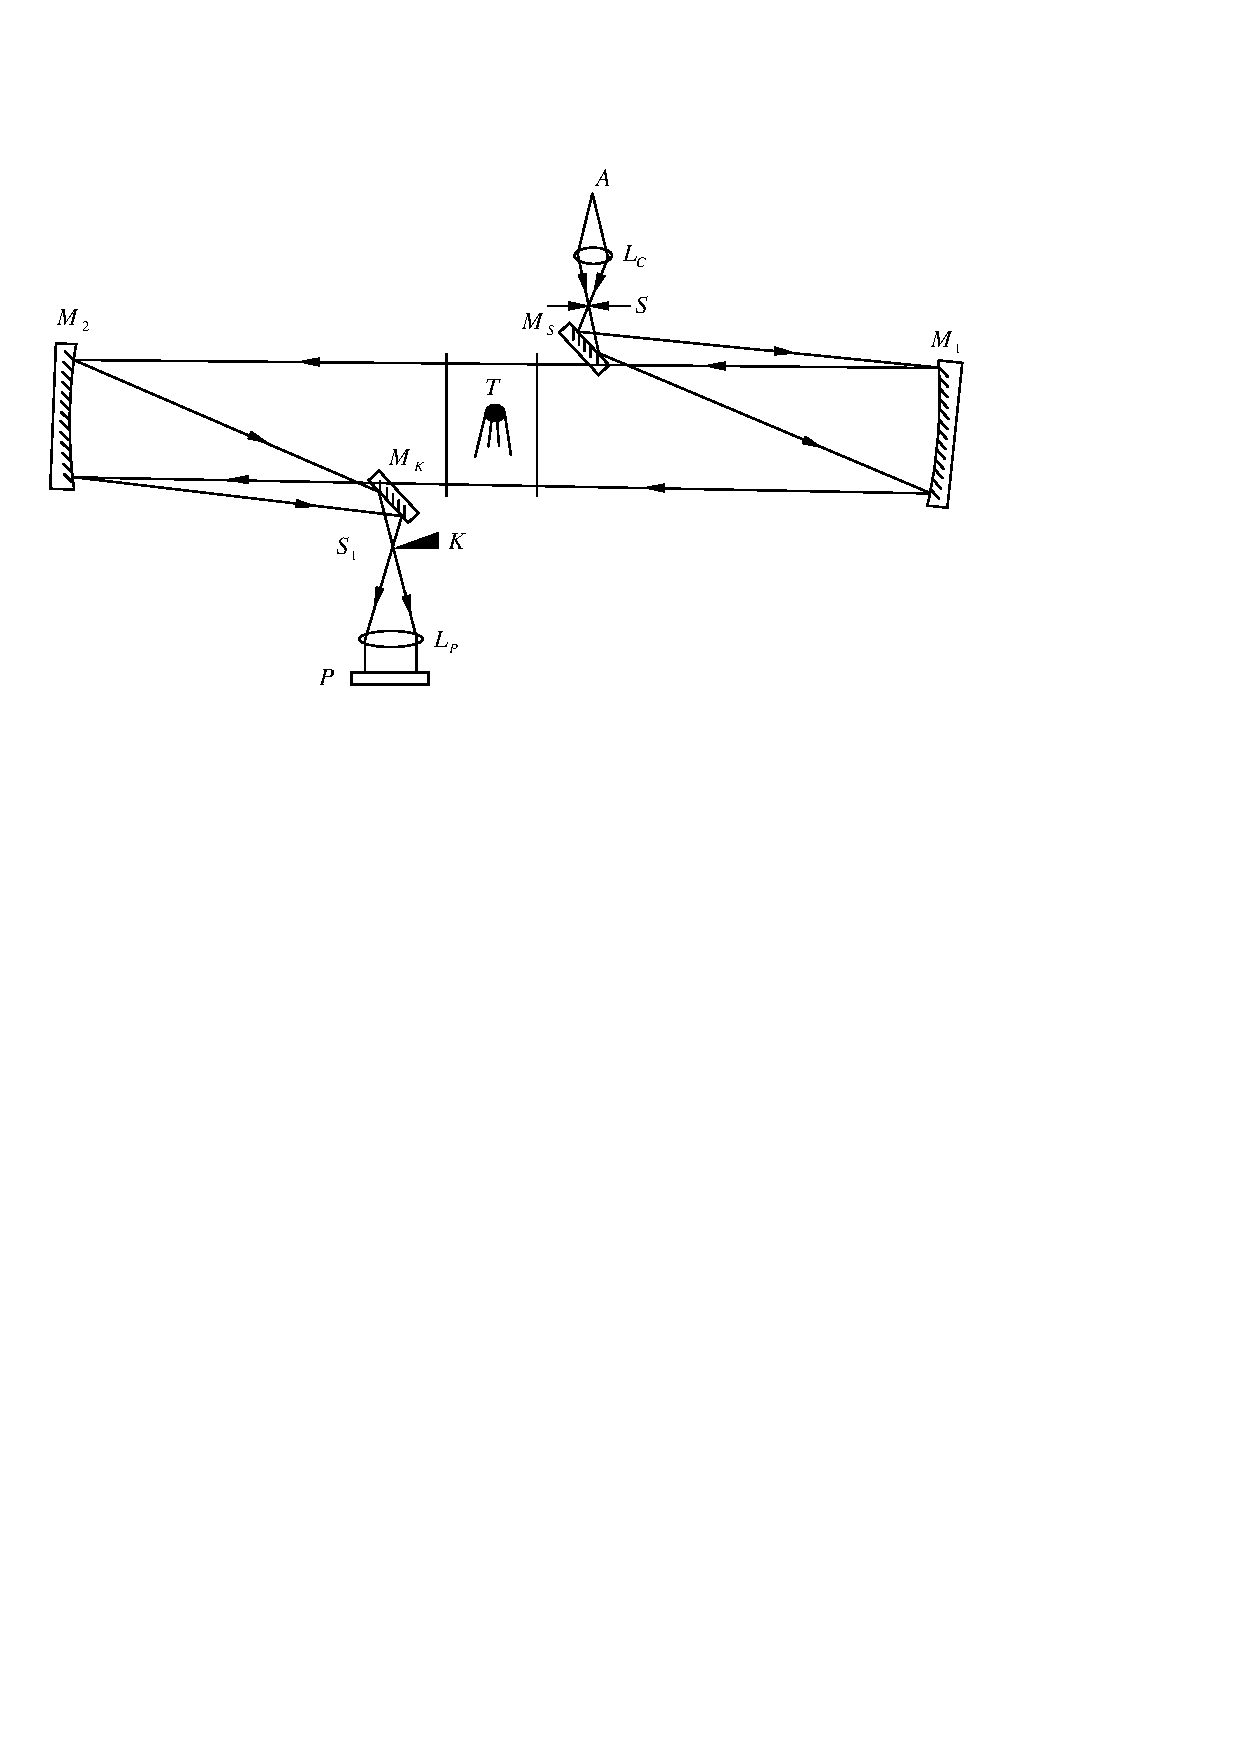
\includegraphics[width=0.85\textwidth]{schlieren.pdf}\\
\textcolor{blue}{双镜平行光纹影系统}
\end{center}
}

\section{实验结果与分析}
\subsection{实验结果}

%\frame{\frametitle{火焰图案(视频)}
%\includemovie[poster, autostart, mouse, repeat]{4.2in}{1.2in}{./avi/fire.avi}
%}

\frame[<+->]{\frametitle{火焰图案}
\begin{minipage}[b]{.5\textwidth}
\centering
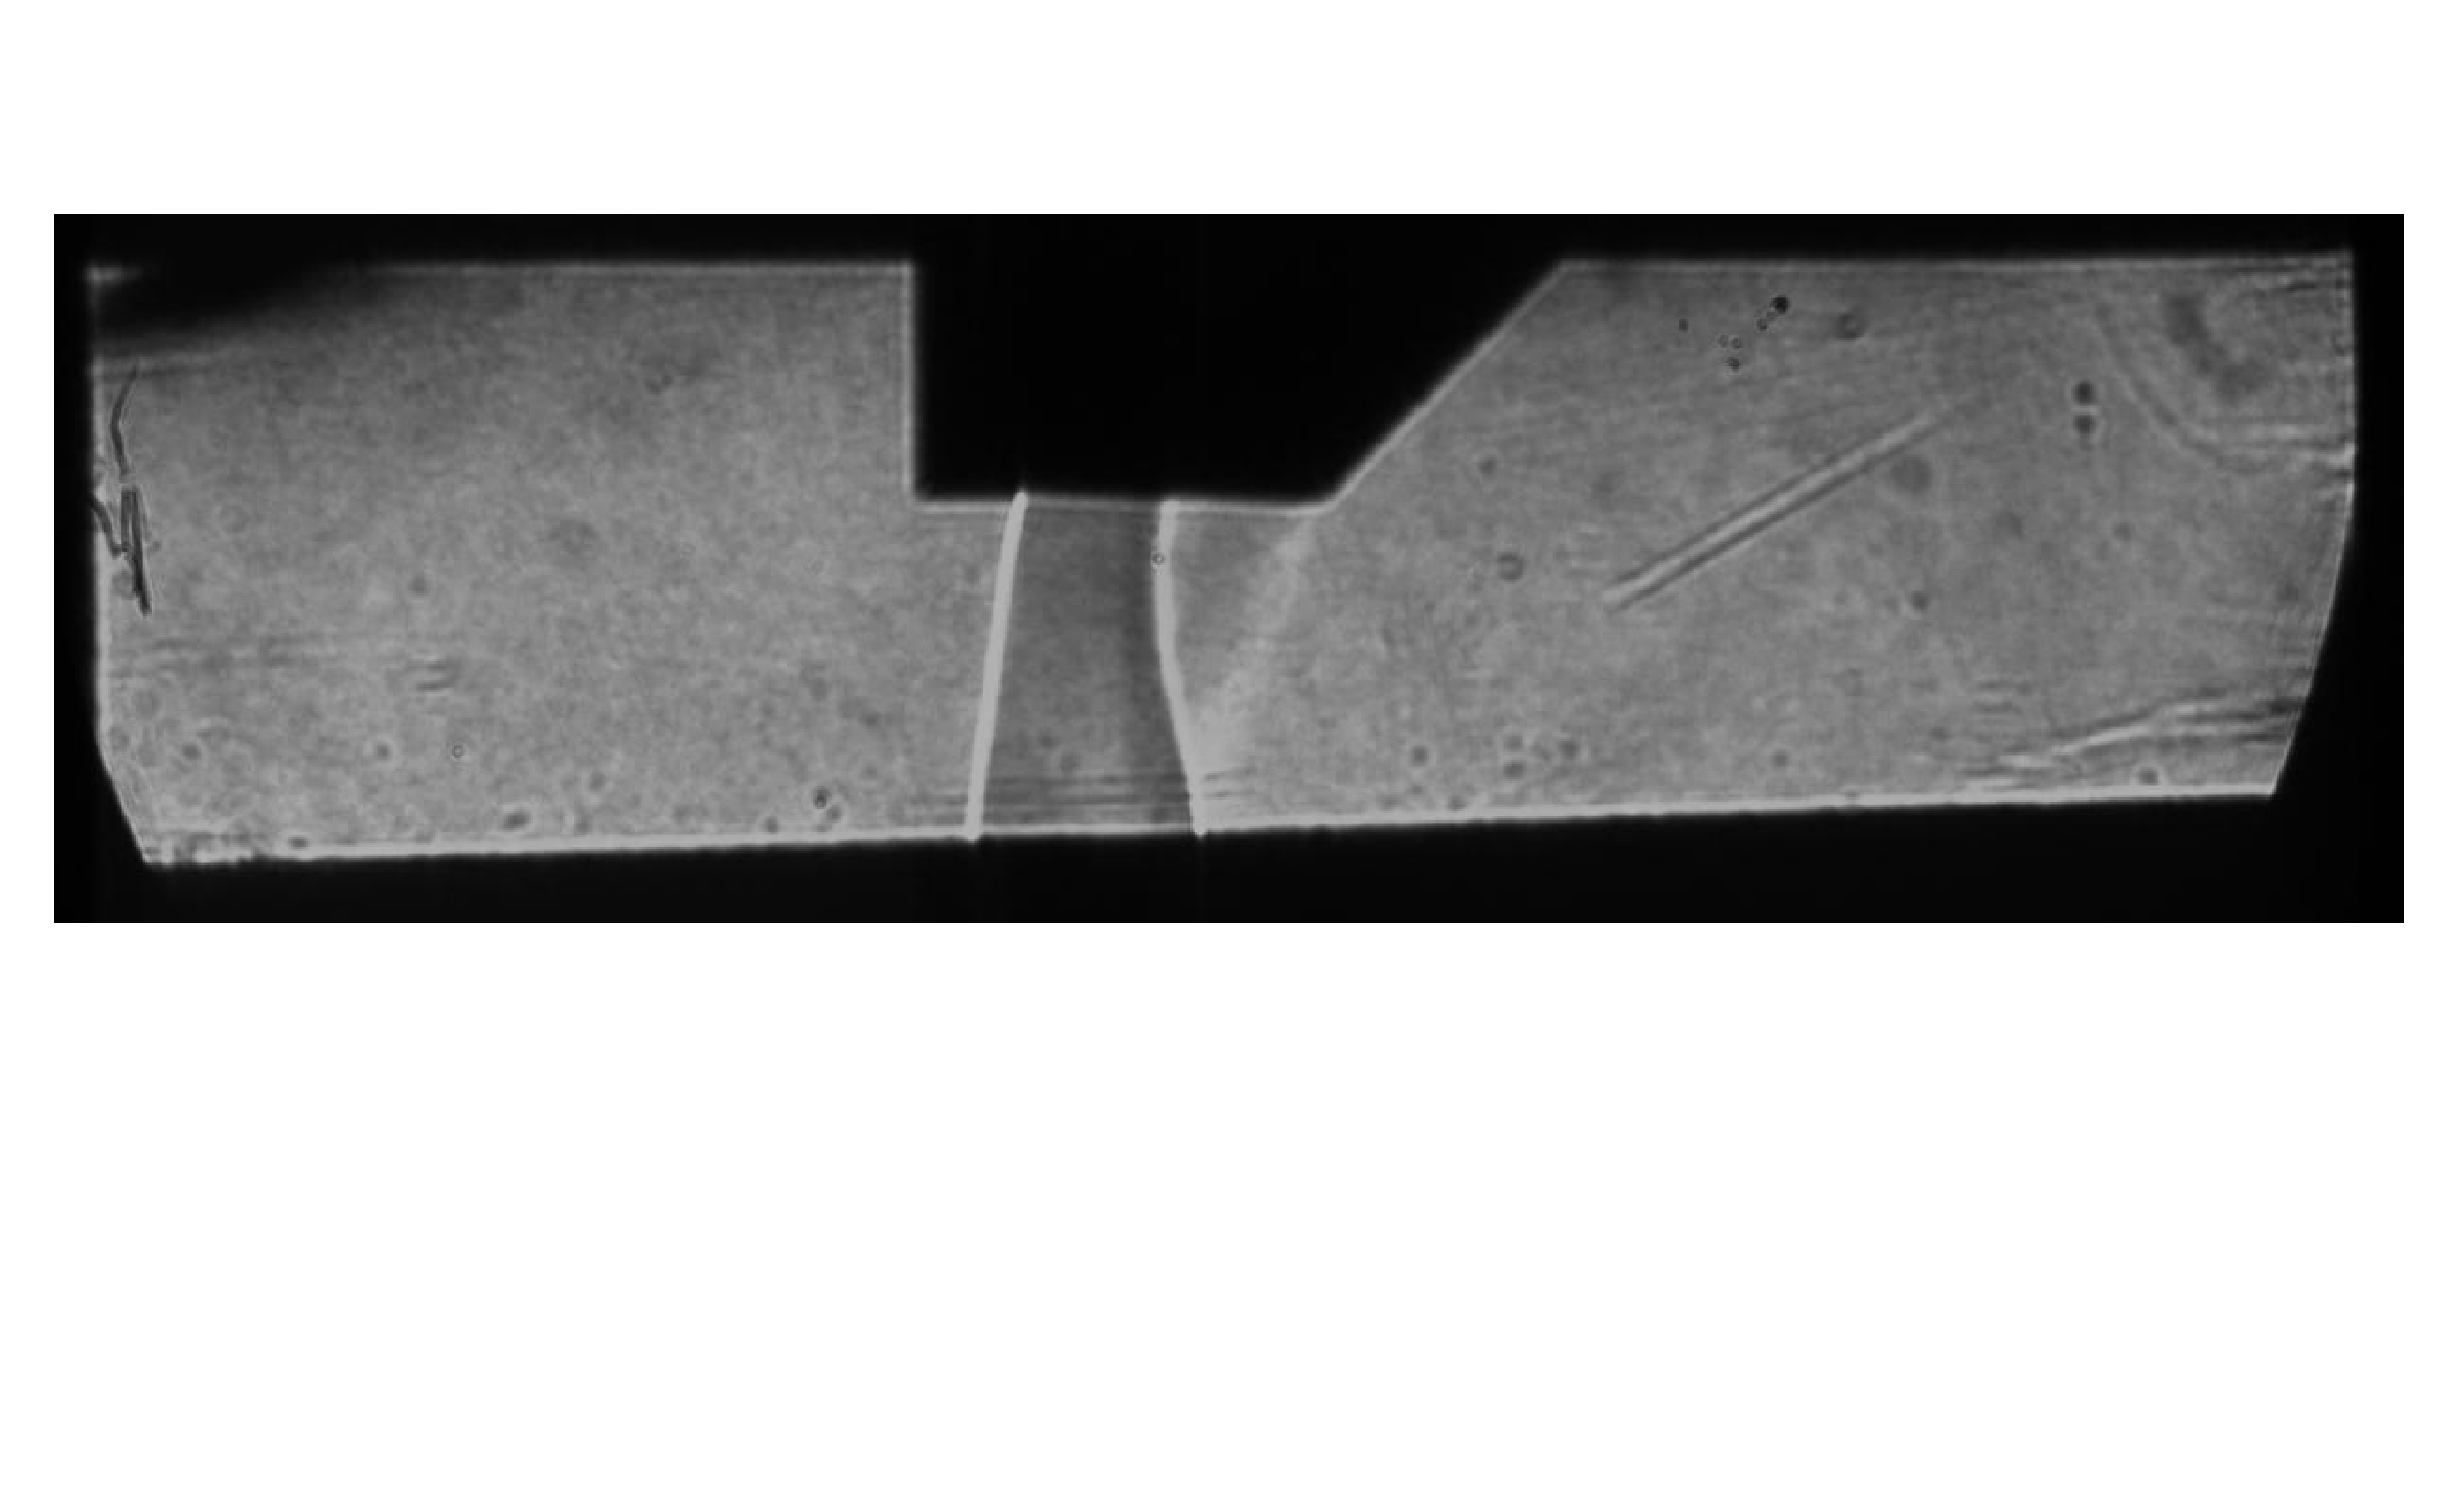
\includegraphics[width=0.99\textwidth]{shadow1of2.pdf}\\
(a)阴影法{\textcolor{white}{纵切1/2光线}}
\end{minipage}%
\begin{minipage}[b]{.5\textwidth}
\centering
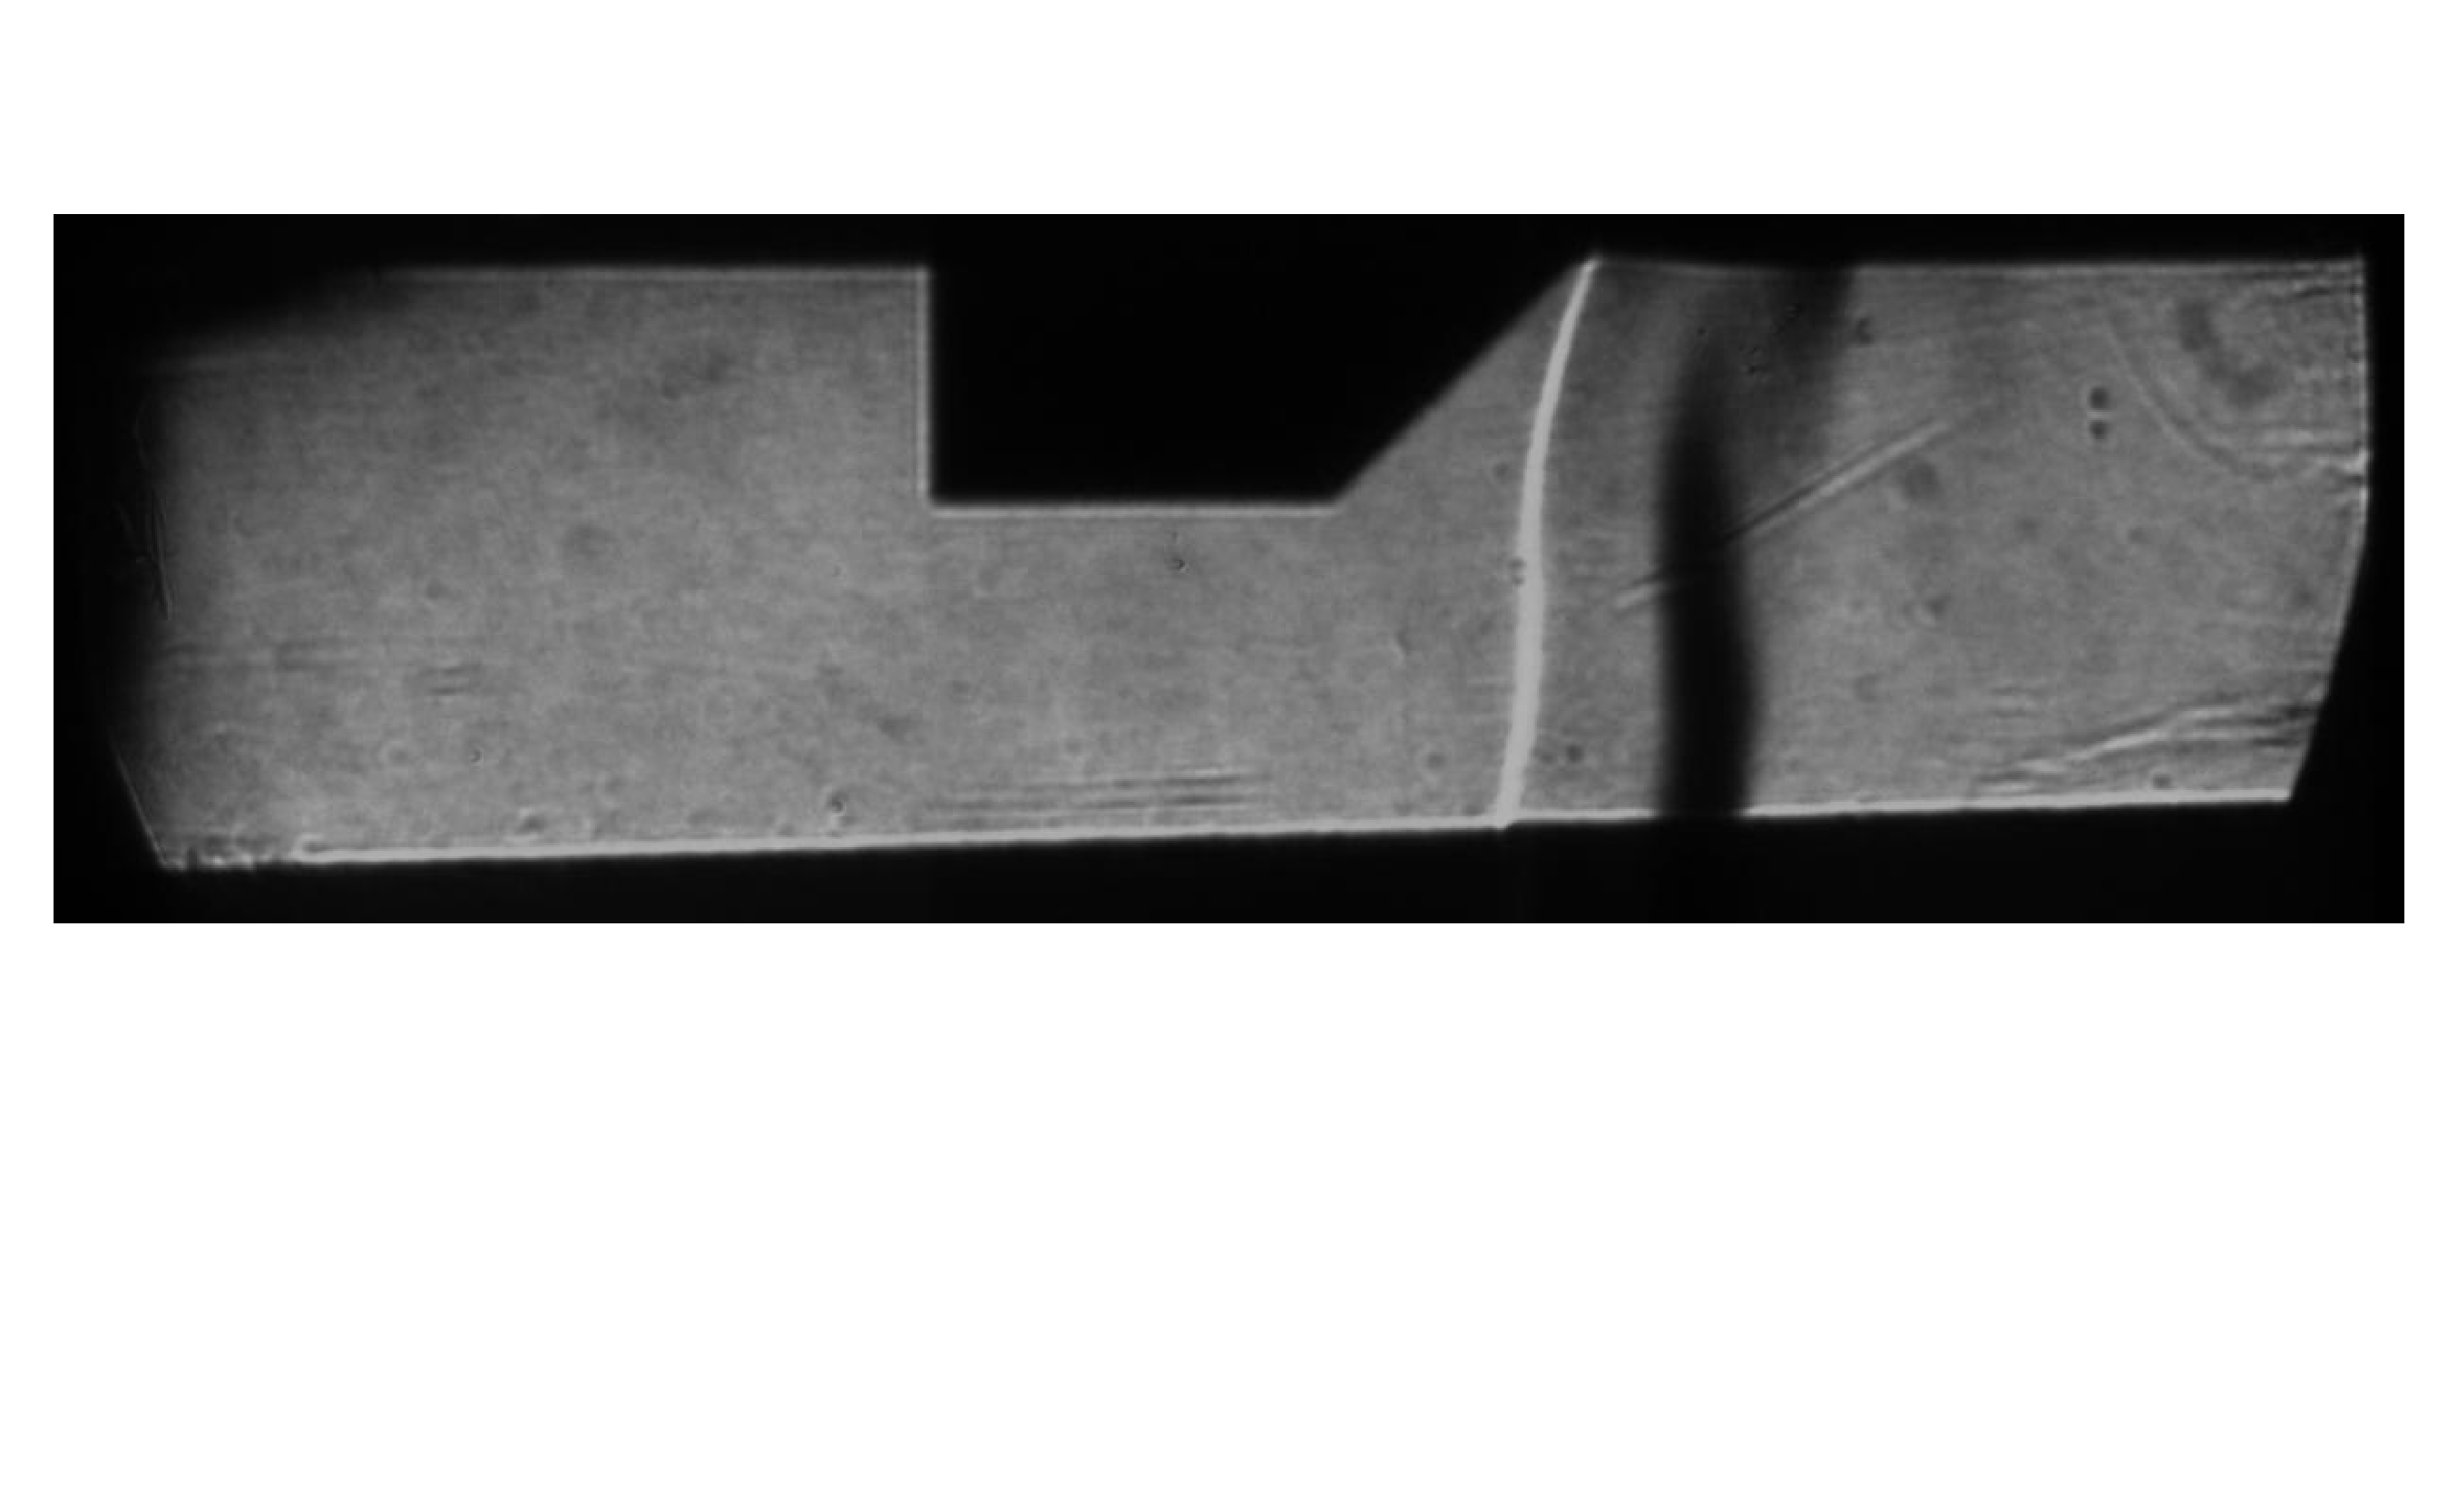
\includegraphics[width=0.99\textwidth]{fire-schlieren1of2.pdf}\\
(b)纹影法纵切1/2光线
\end{minipage}
\vspace{1em}

\begin{minipage}[b]{.5\textwidth}
\centering
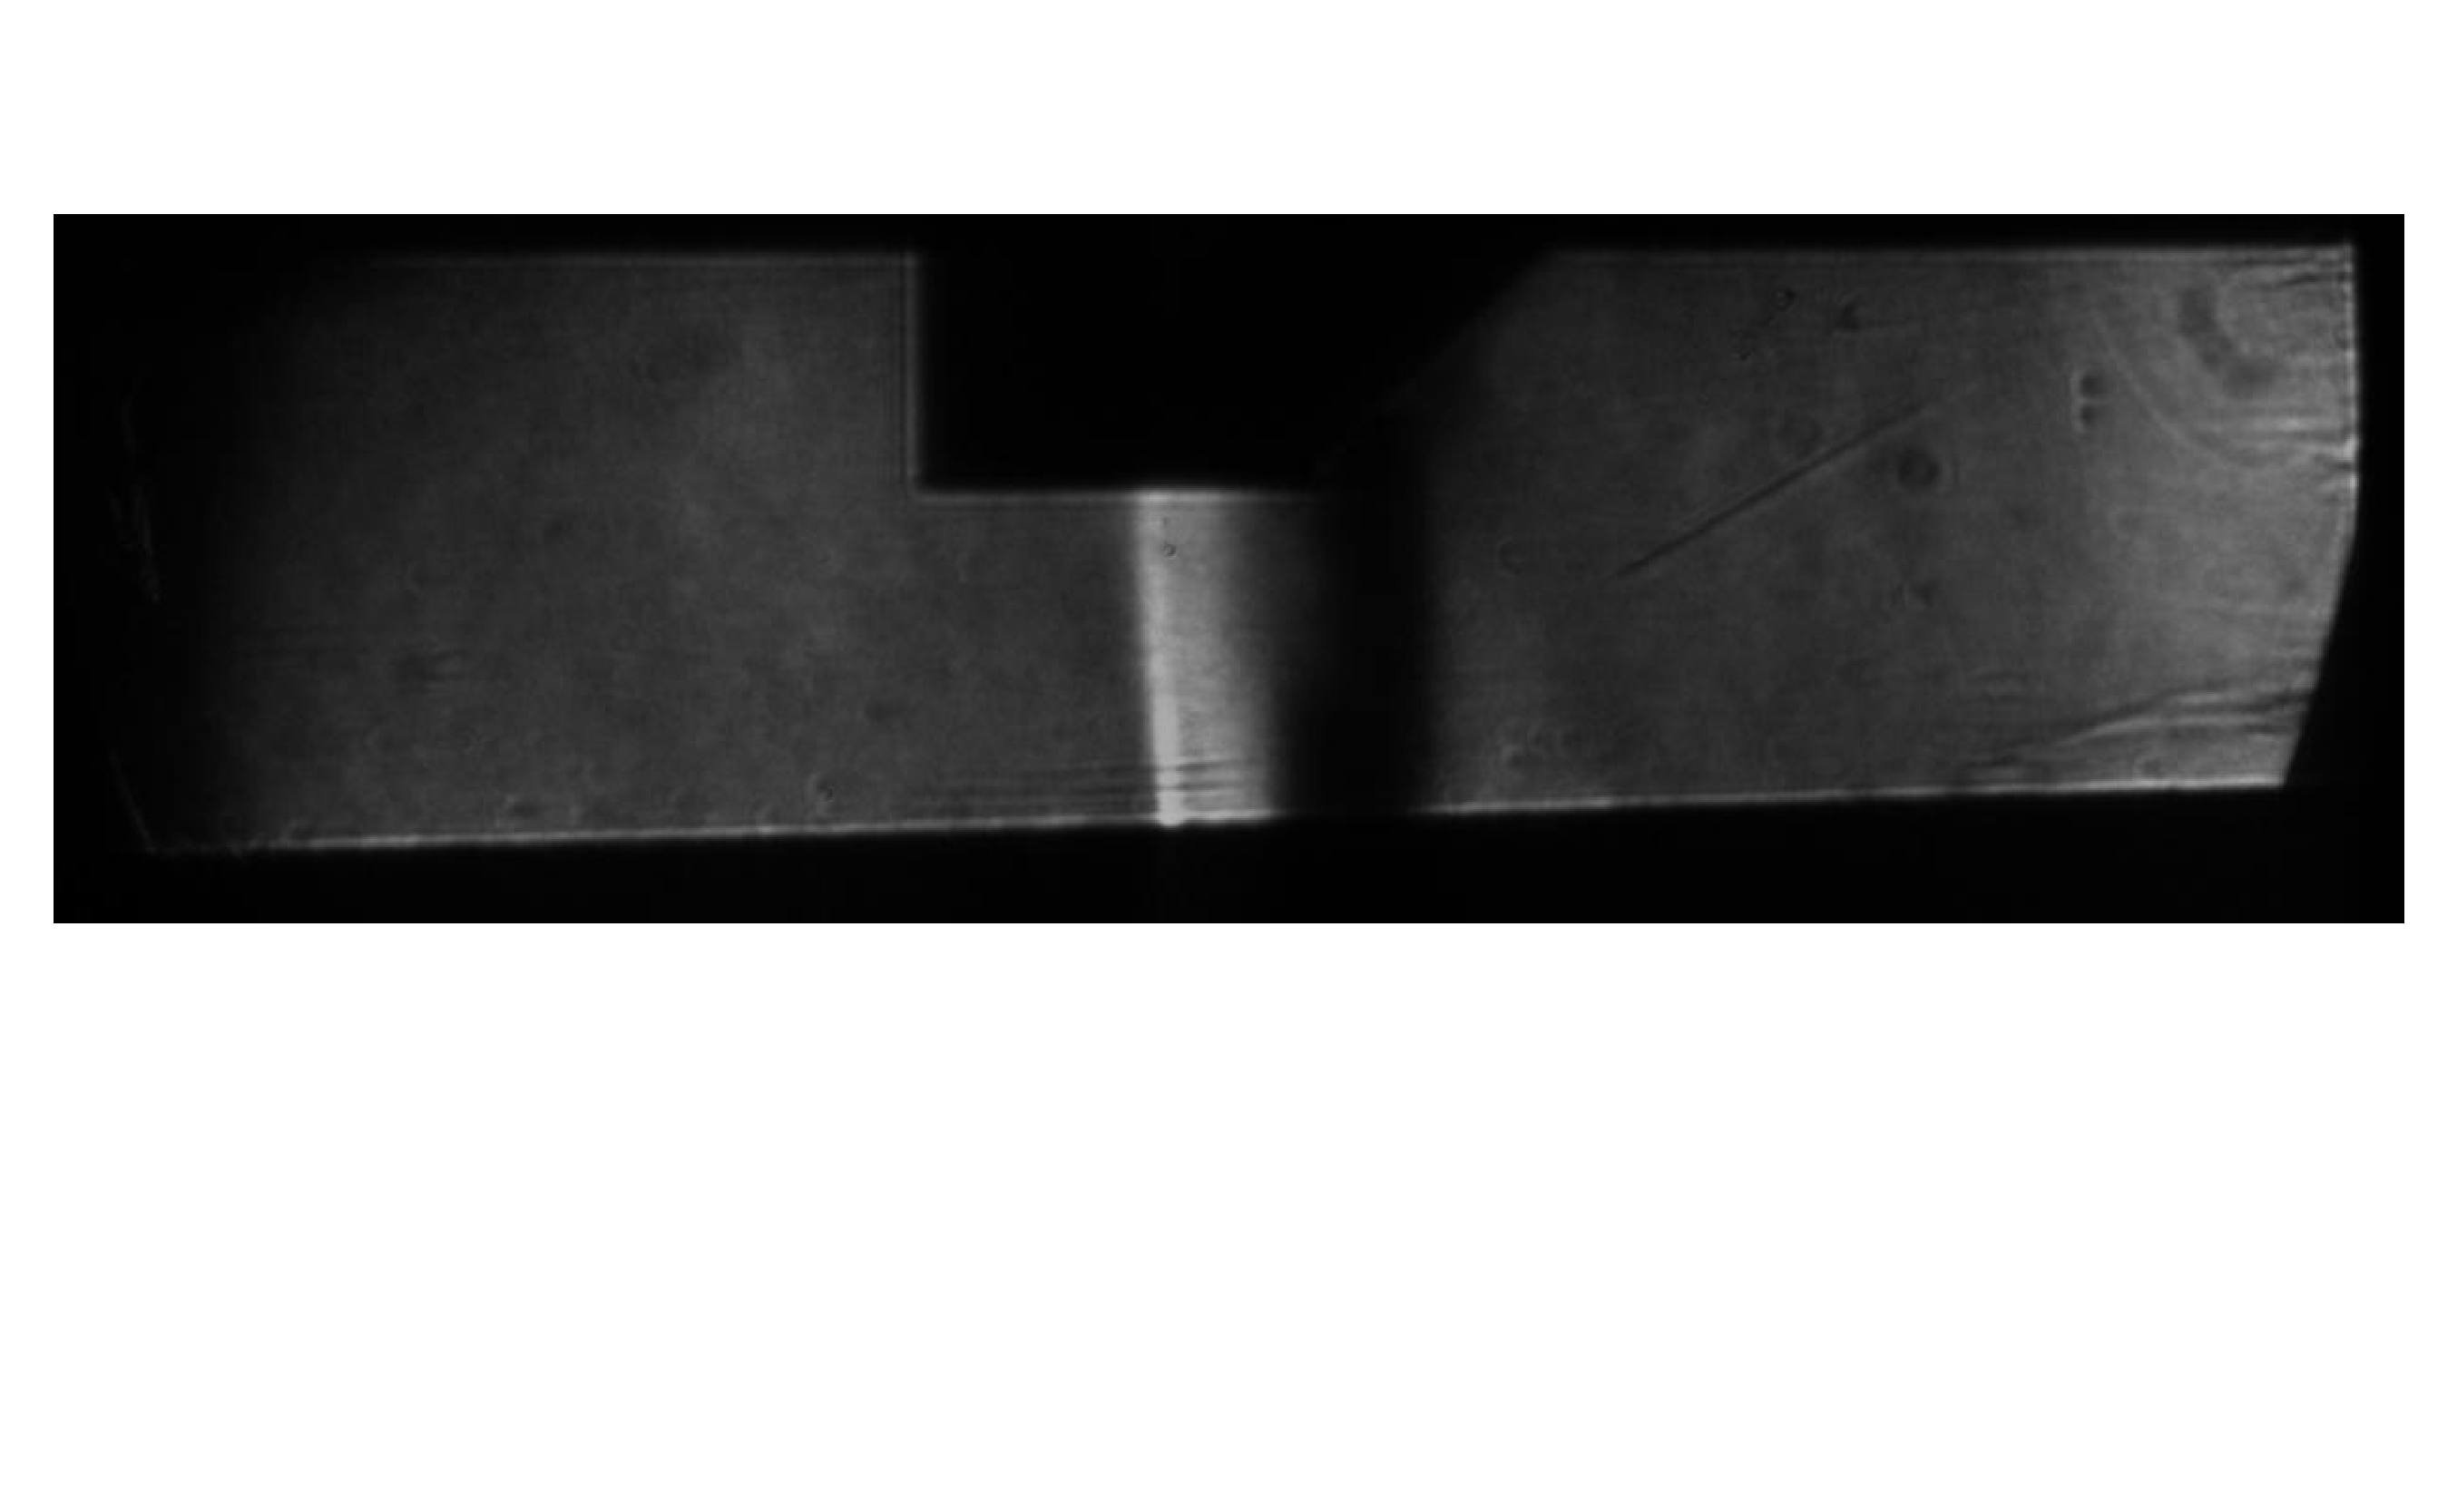
\includegraphics[width=0.99\textwidth]{fire-schlieren3of4.pdf}\\
(c)纹影法纵切3/4光线
\end{minipage}%
\begin{minipage}[b]{.5\textwidth}
\centering
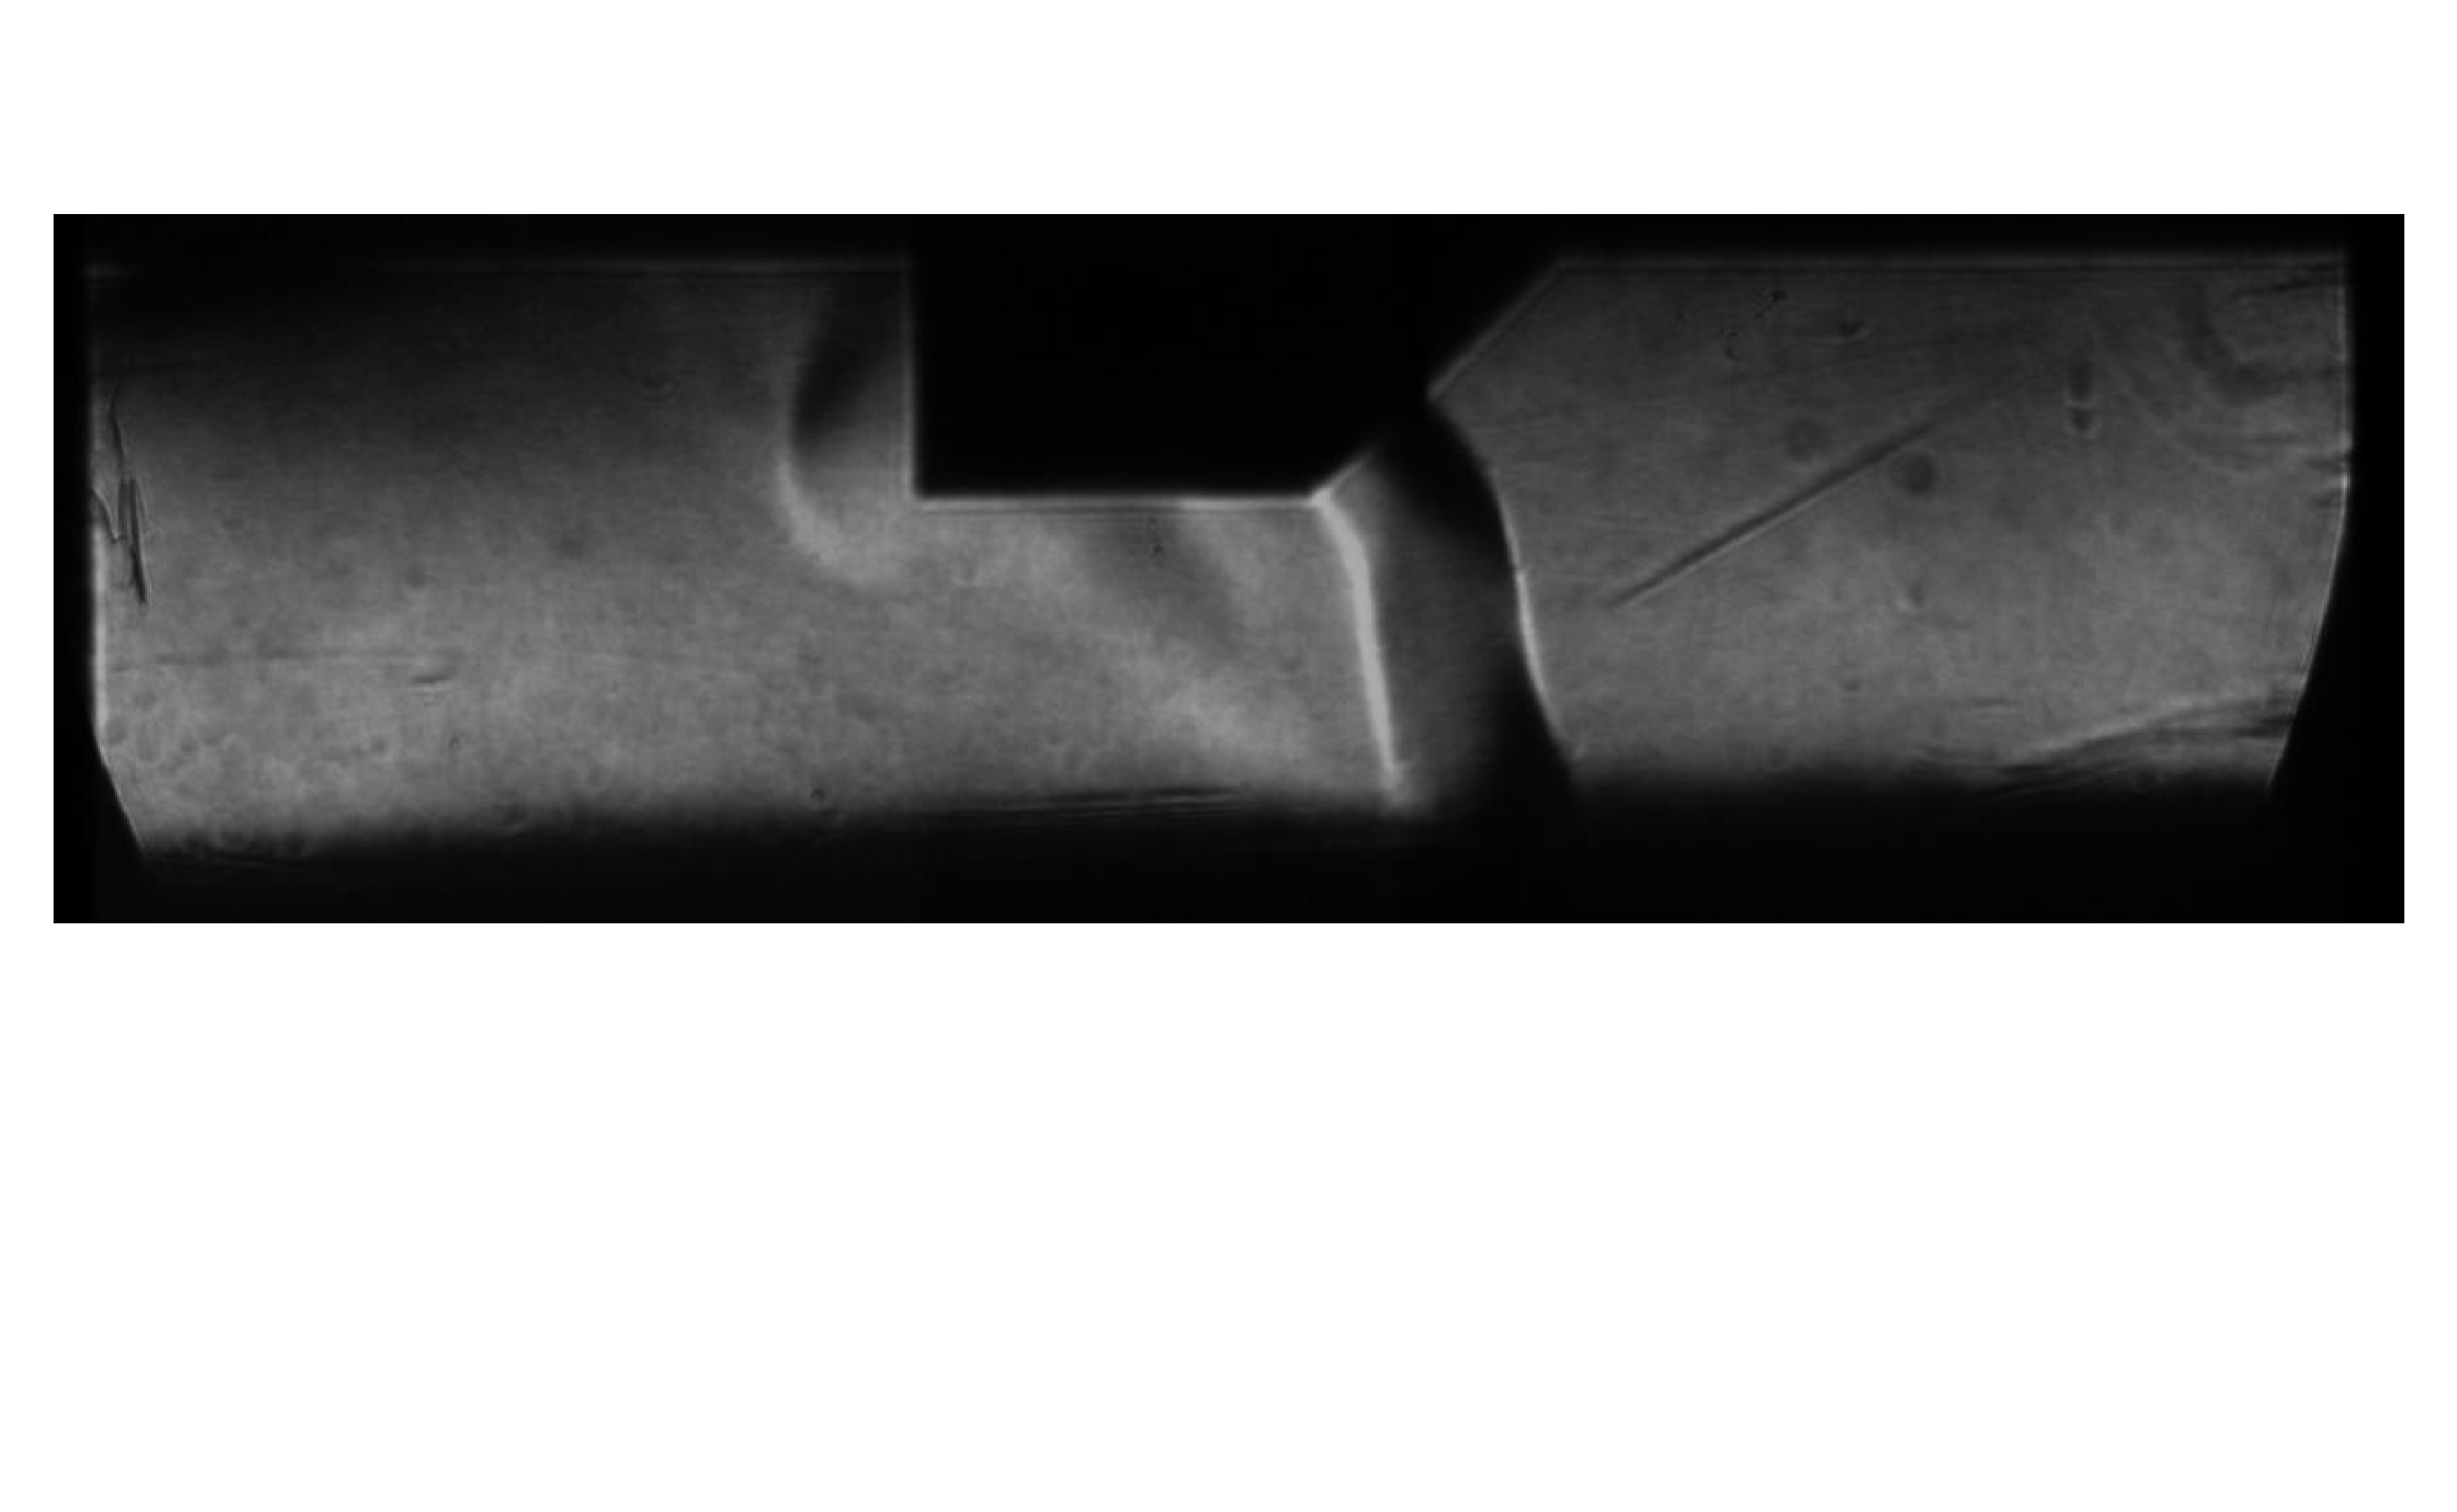
\includegraphics[width=0.99\textwidth]{fire-hschlieren1of2.pdf}\\
(d)纹影法横切1/2光线
\end{minipage}
}

%\frame{\frametitle{激波图案(视频)}
%\includemovie[poster, autostart, mouse, repeat]{4.2in}{1.2in}{./avi/wave.avi}
%\includemovie[poster, autostart, mouse]{4.2in}{1.2in}{./avi/wave.avi}
%}

\frame[<+->]{\frametitle{激波图案}
\begin{minipage}[b]{.5\textwidth}
\centering
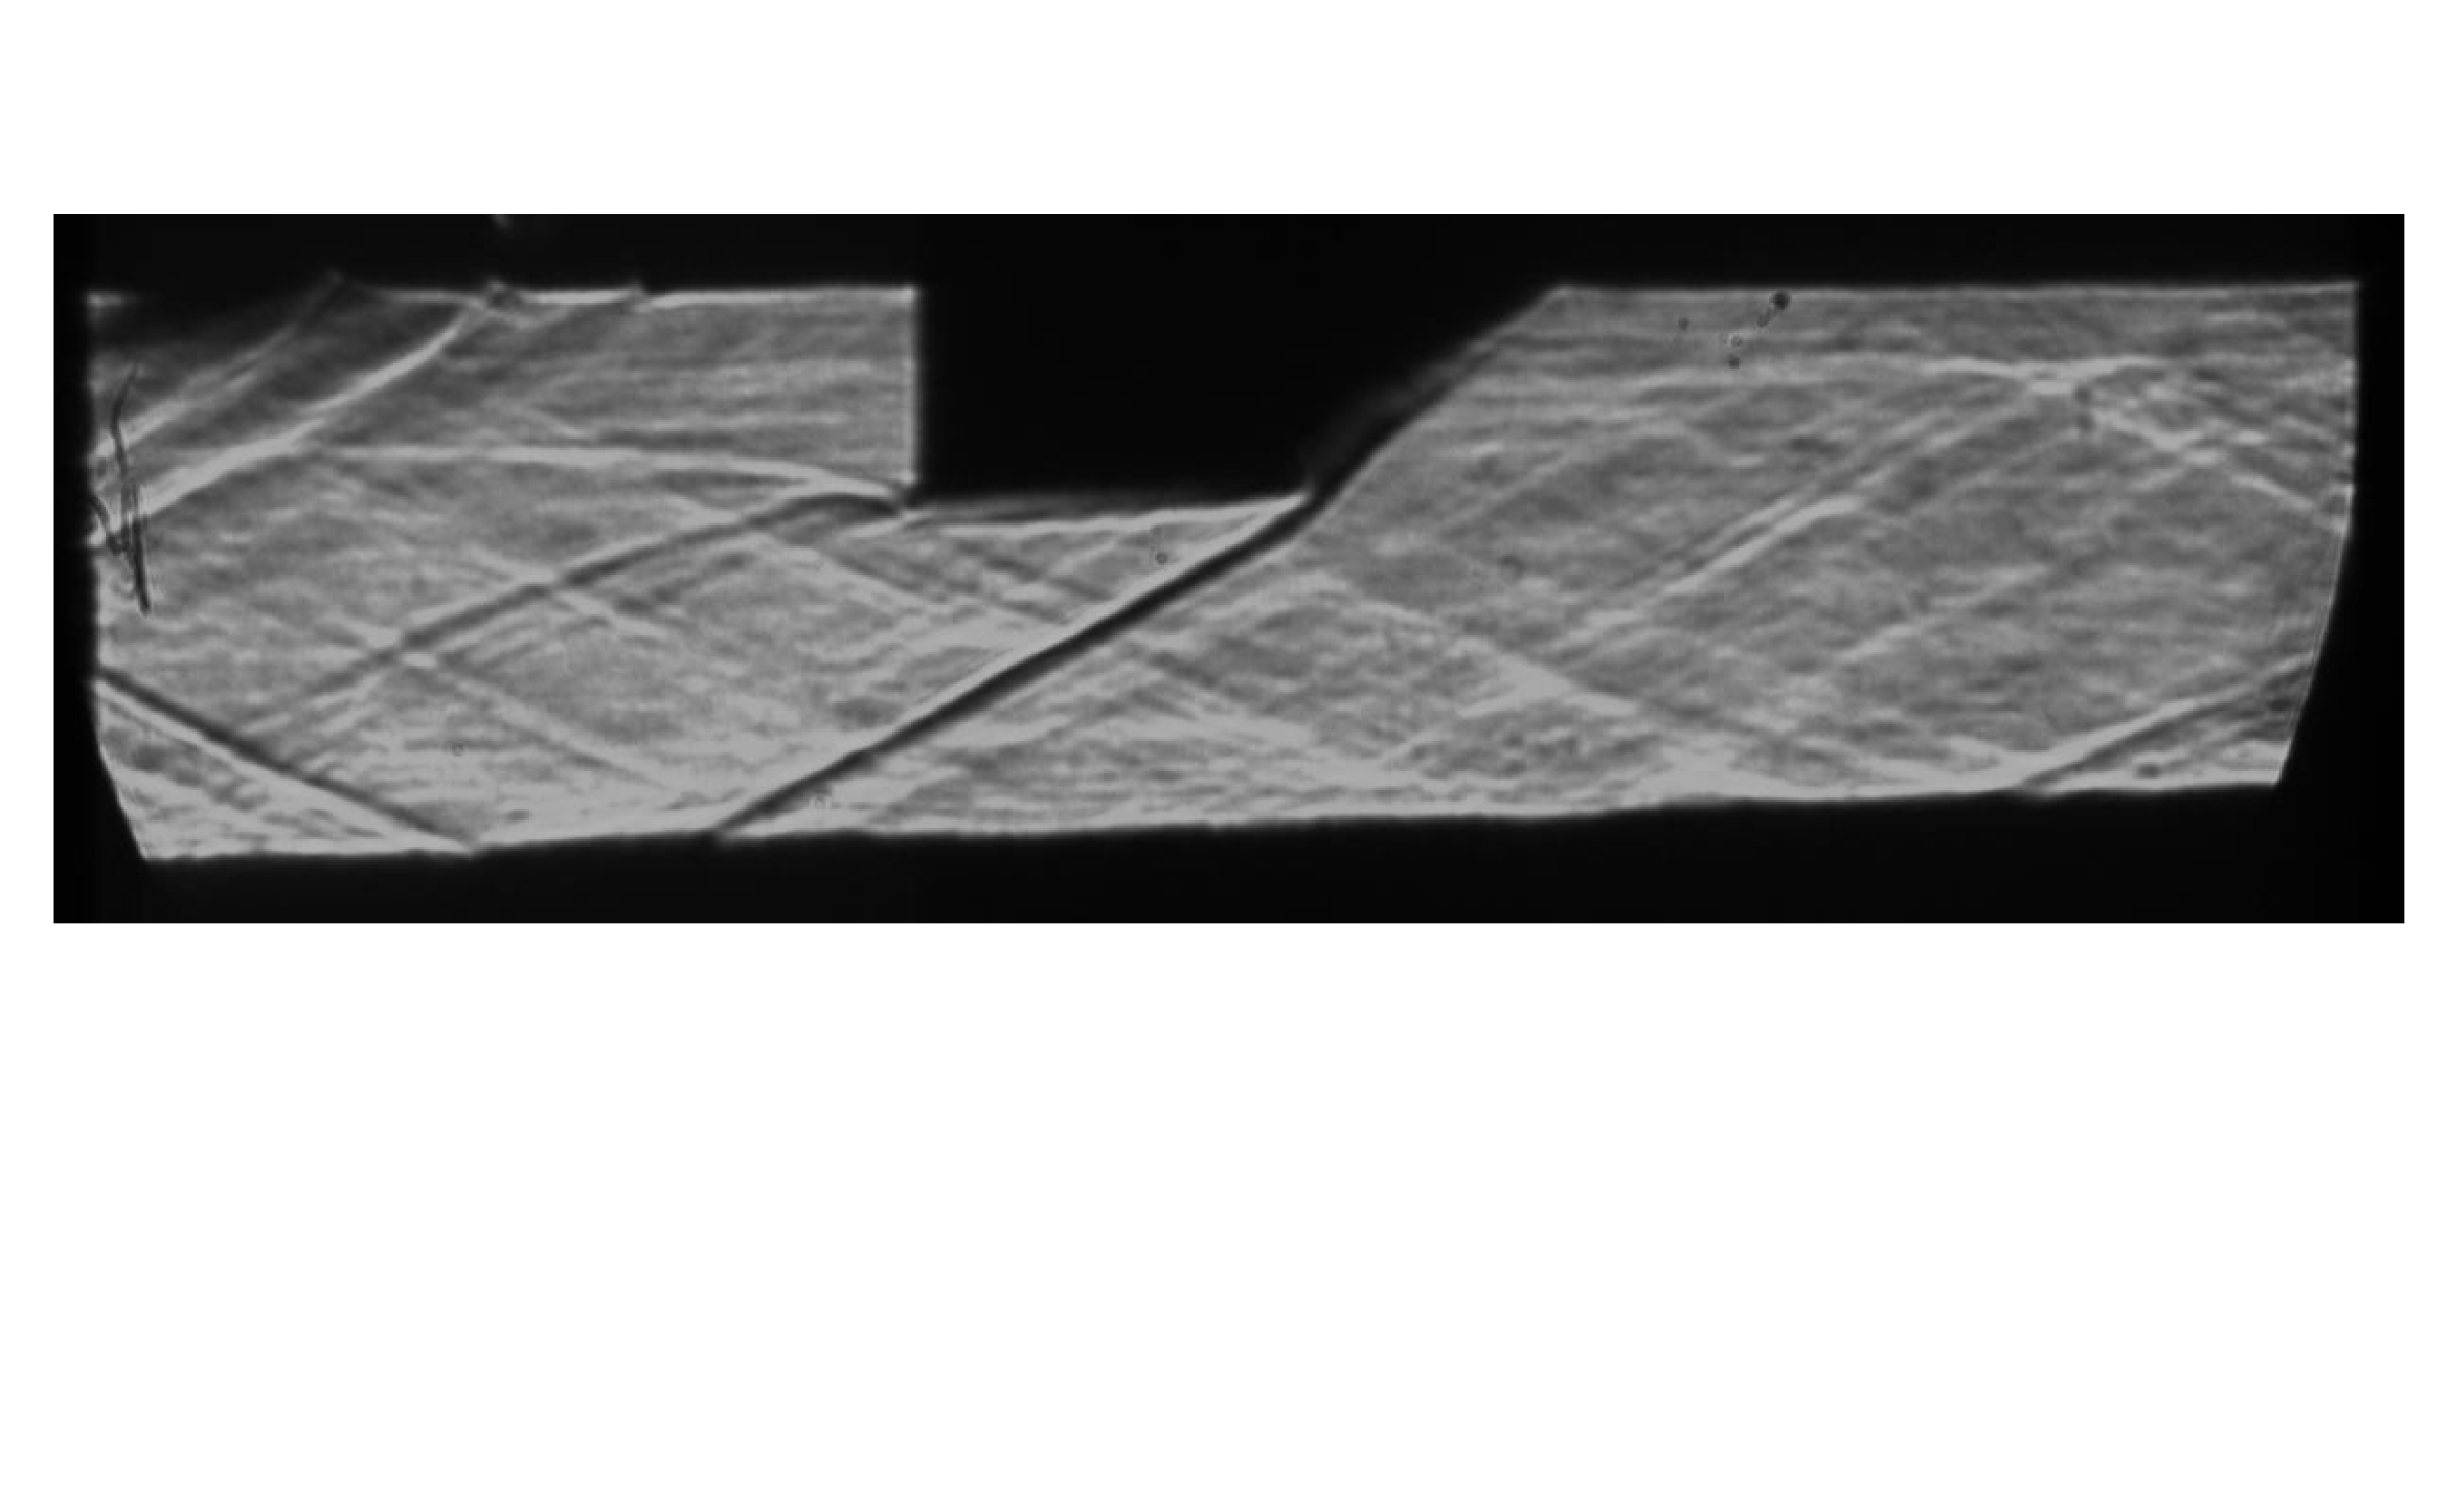
\includegraphics[width=0.99\textwidth]{WaveShadow.pdf}\\
(a)阴影法{\textcolor{white}{纵切1/2光线}}
\end{minipage}%
\begin{minipage}[b]{.5\textwidth}
\centering
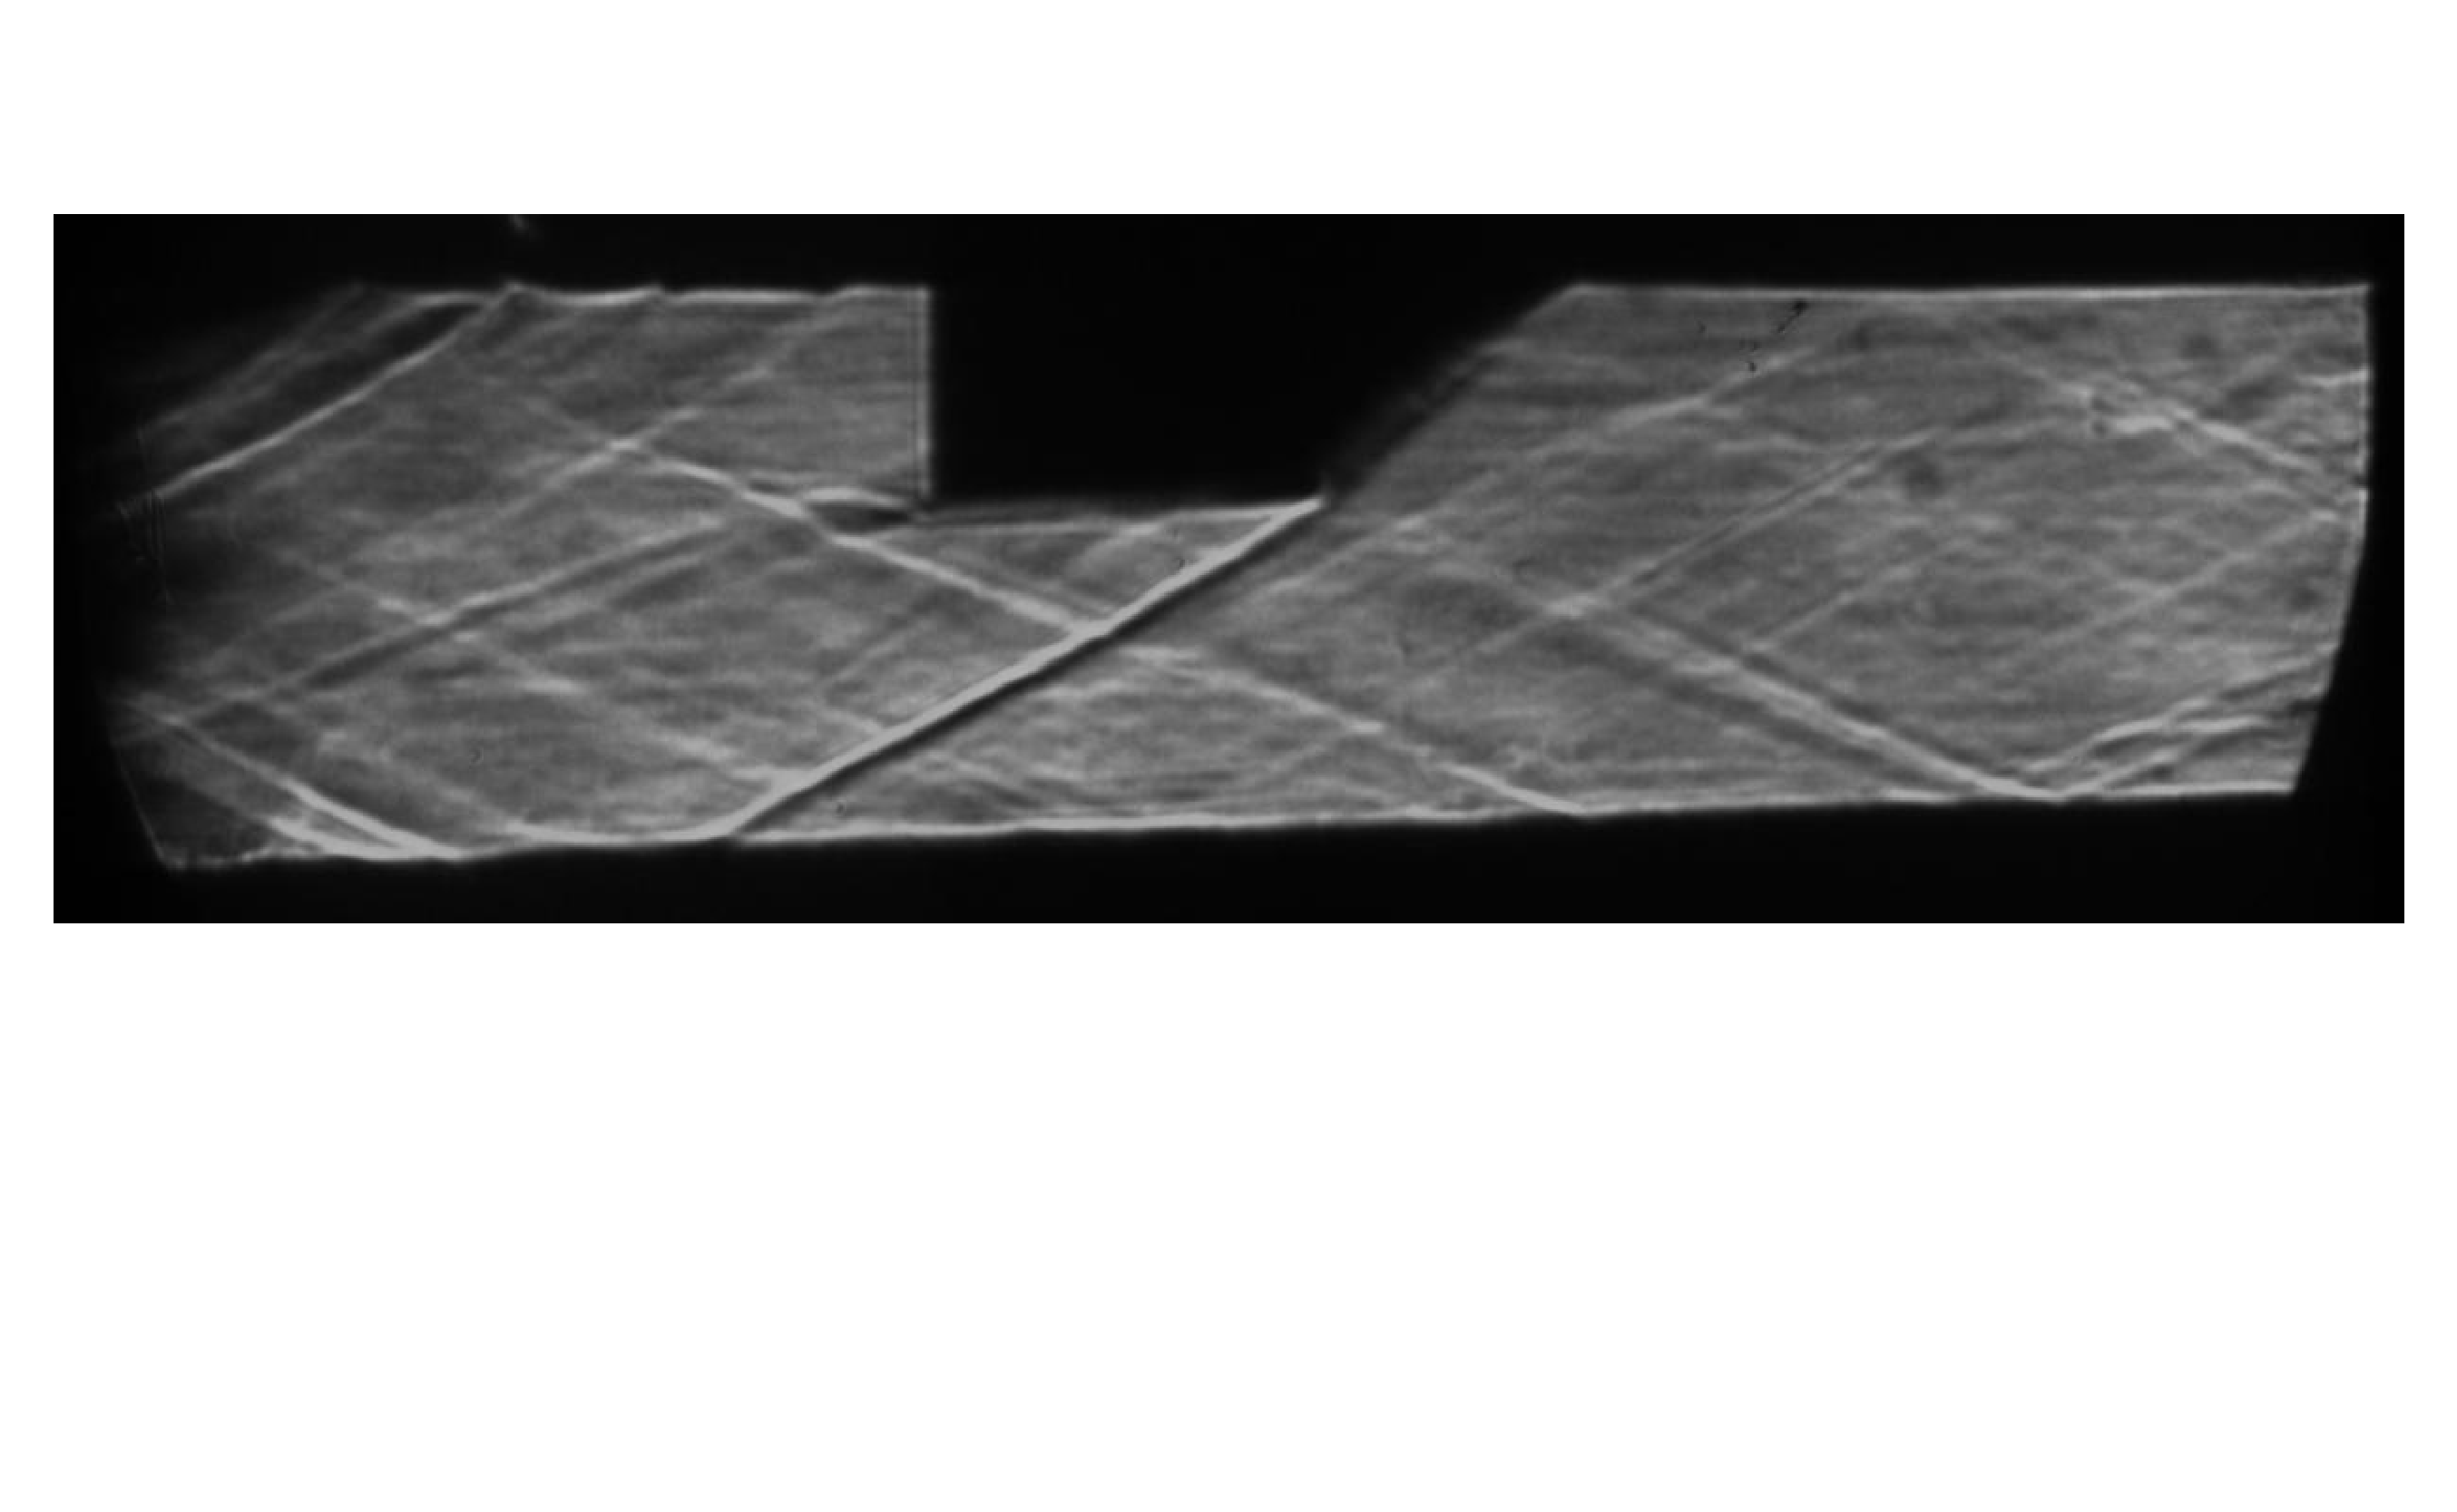
\includegraphics[width=0.99\textwidth]{WaveSchlieren1of2.pdf}\\
(b)纹影法纵切1/2光线
\end{minipage}
\vspace{1em}

\begin{minipage}[b]{.5\textwidth}
\centering
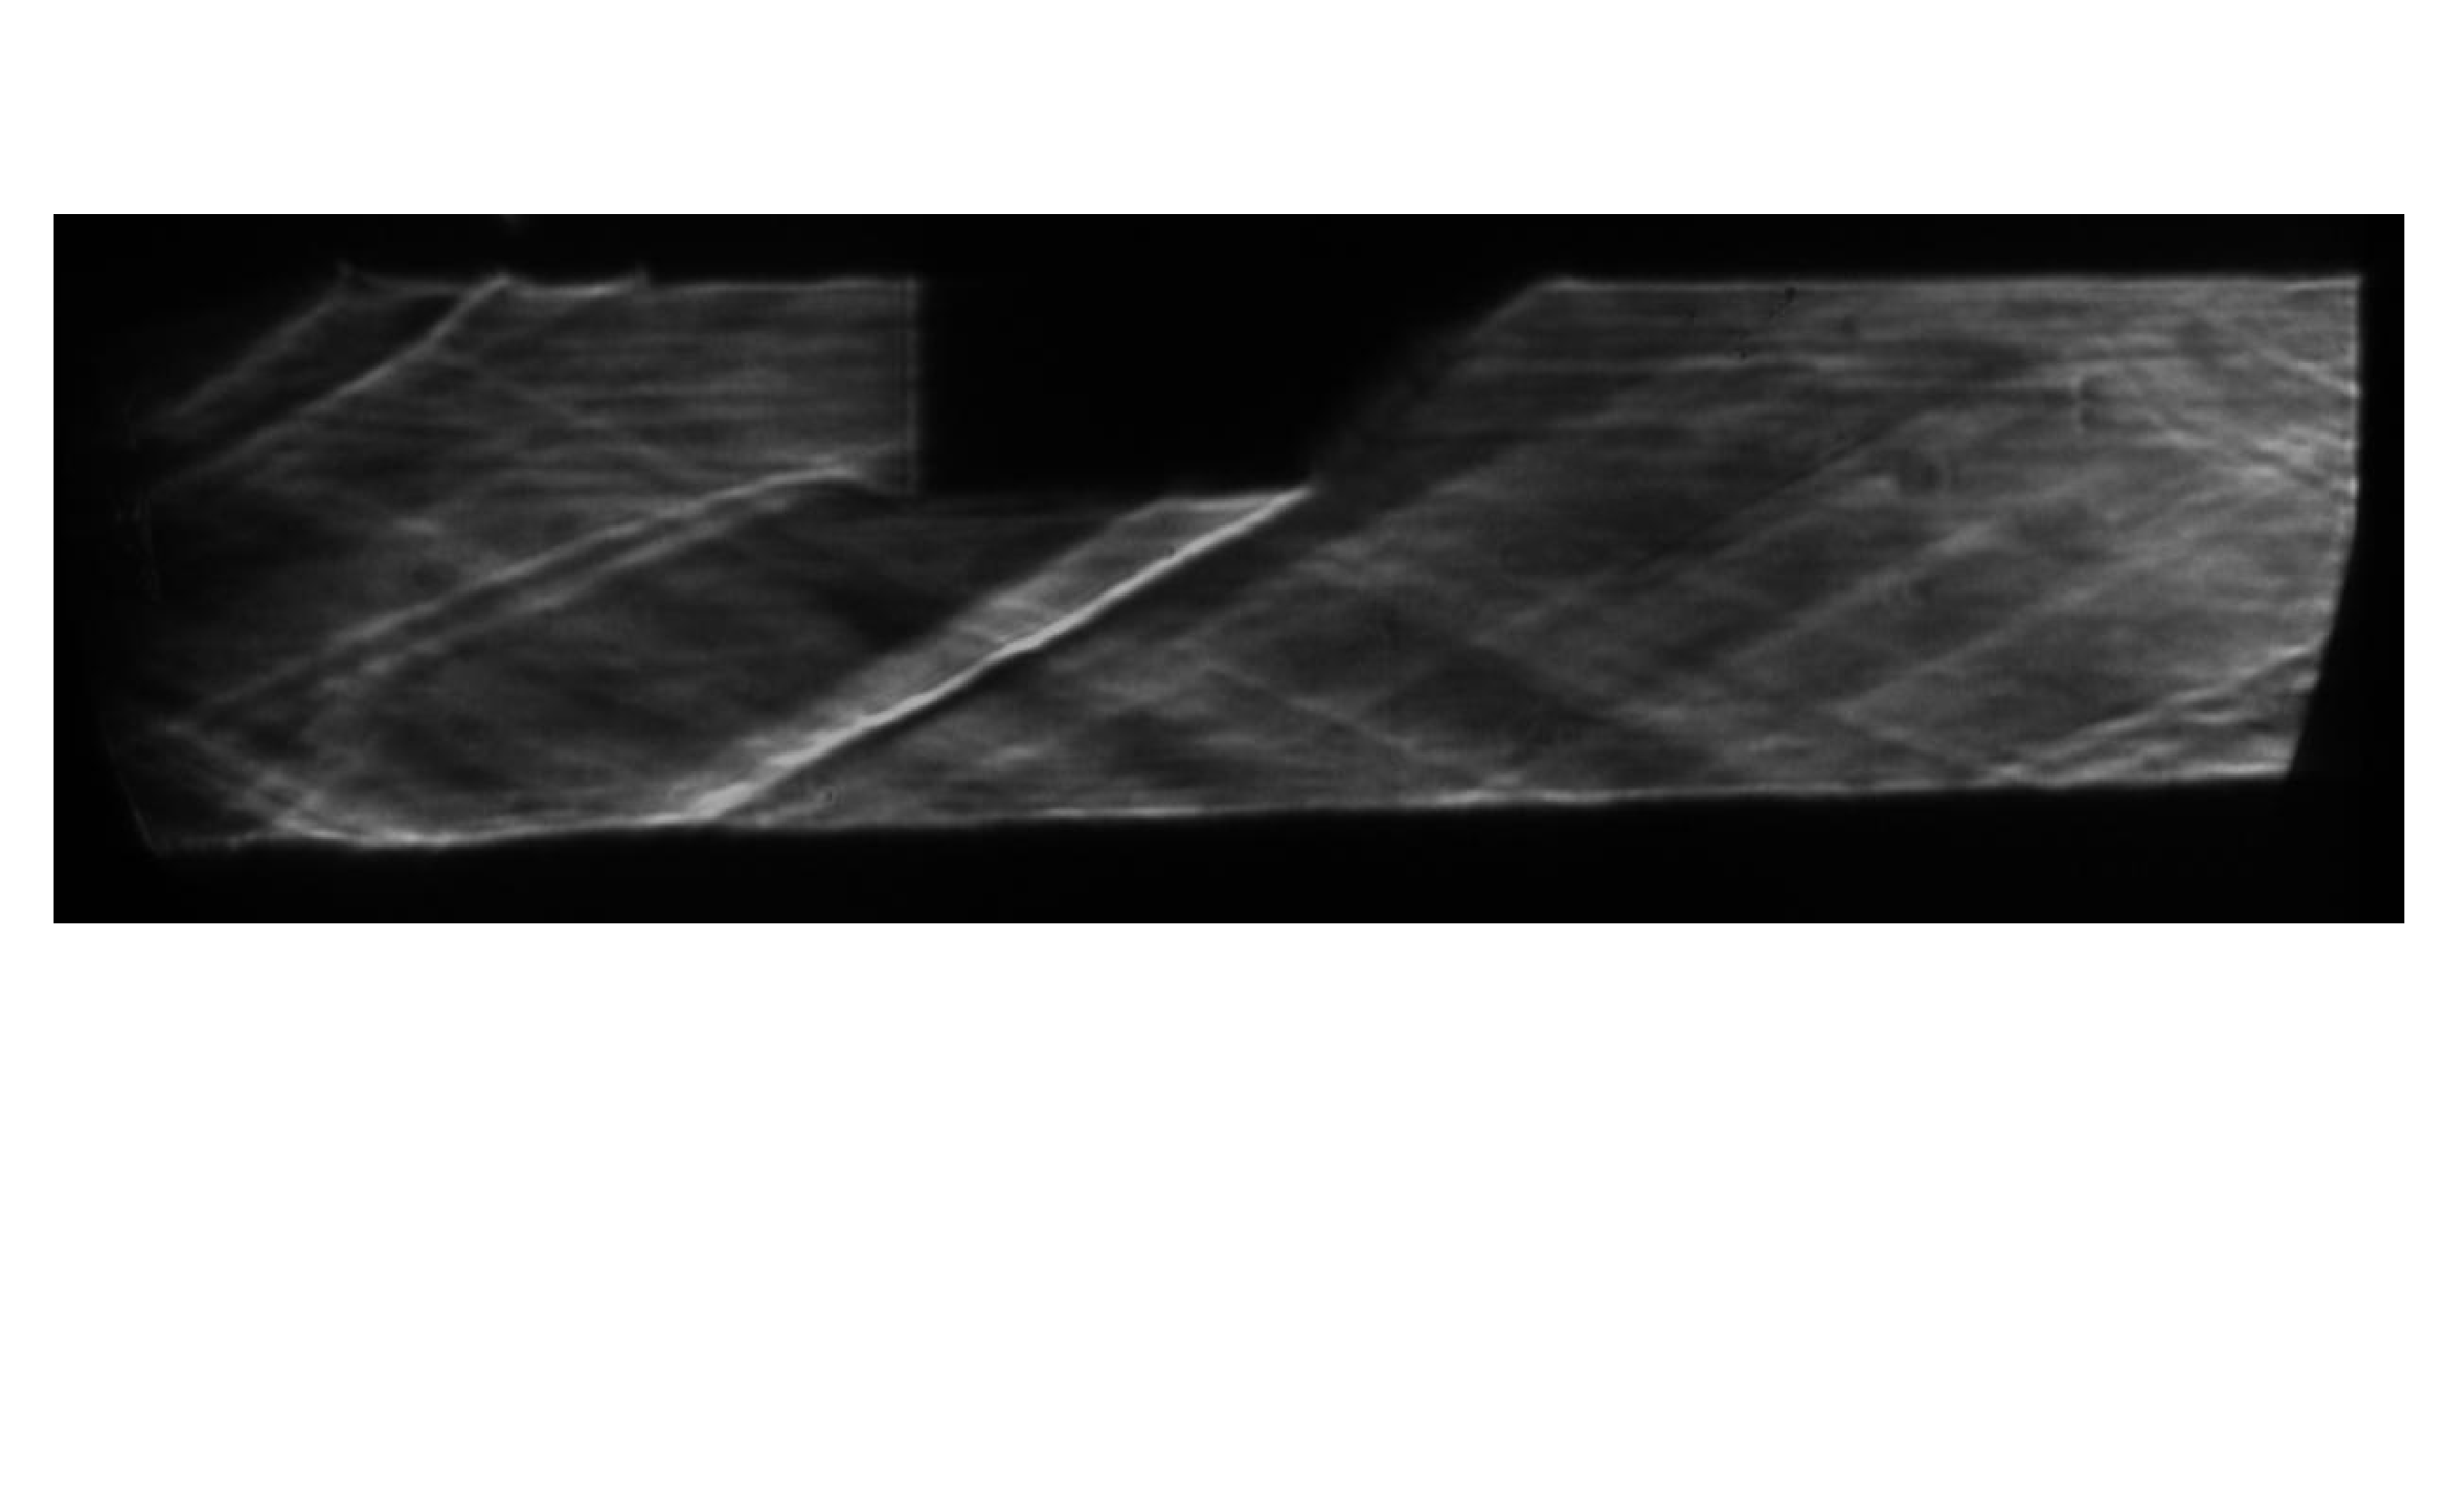
\includegraphics[width=0.99\textwidth]{WaveSchlieren3of4.pdf}\\
(c)纹影法纵切3/4光线
\end{minipage}%
\begin{minipage}[b]{.5\textwidth}
\centering
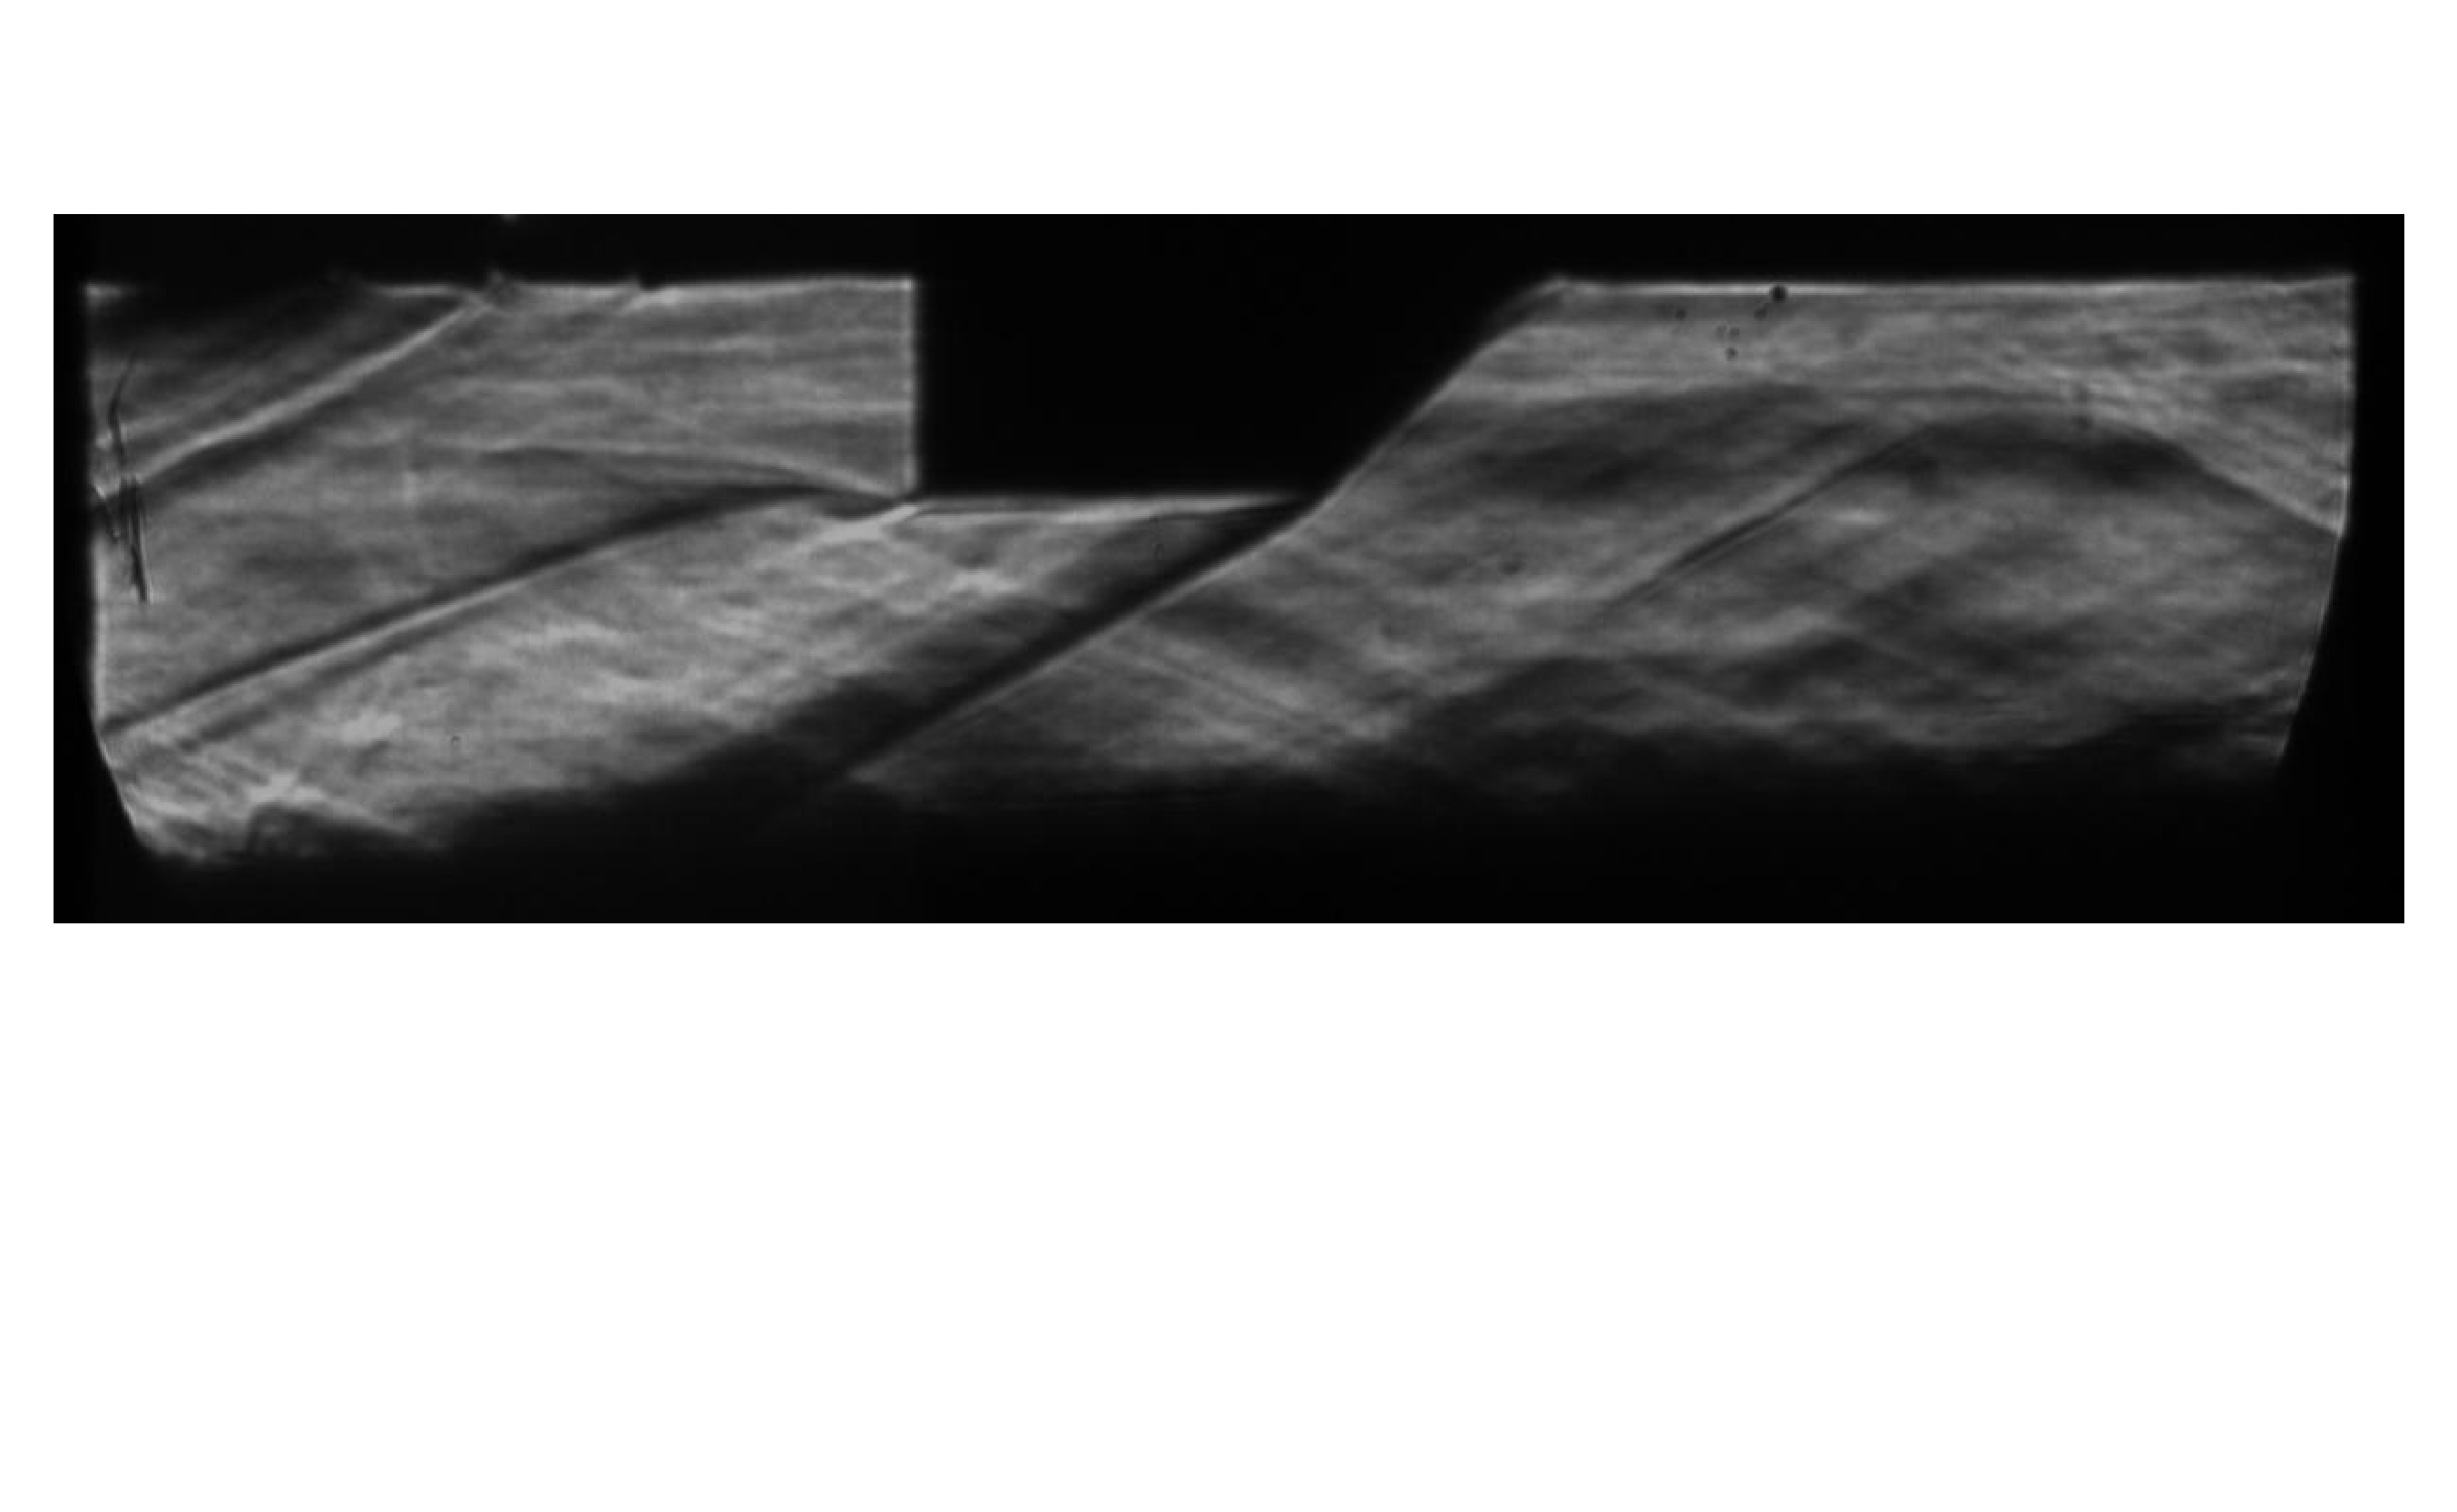
\includegraphics[width=0.99\textwidth]{WaveHSchlieren1of2.pdf}\\
(d)纹影法横切1/2光线
\end{minipage}
}

\subsection{结果分析}
\frame{\frametitle{波的类型与出现原因}
\begin{center}
\fbox{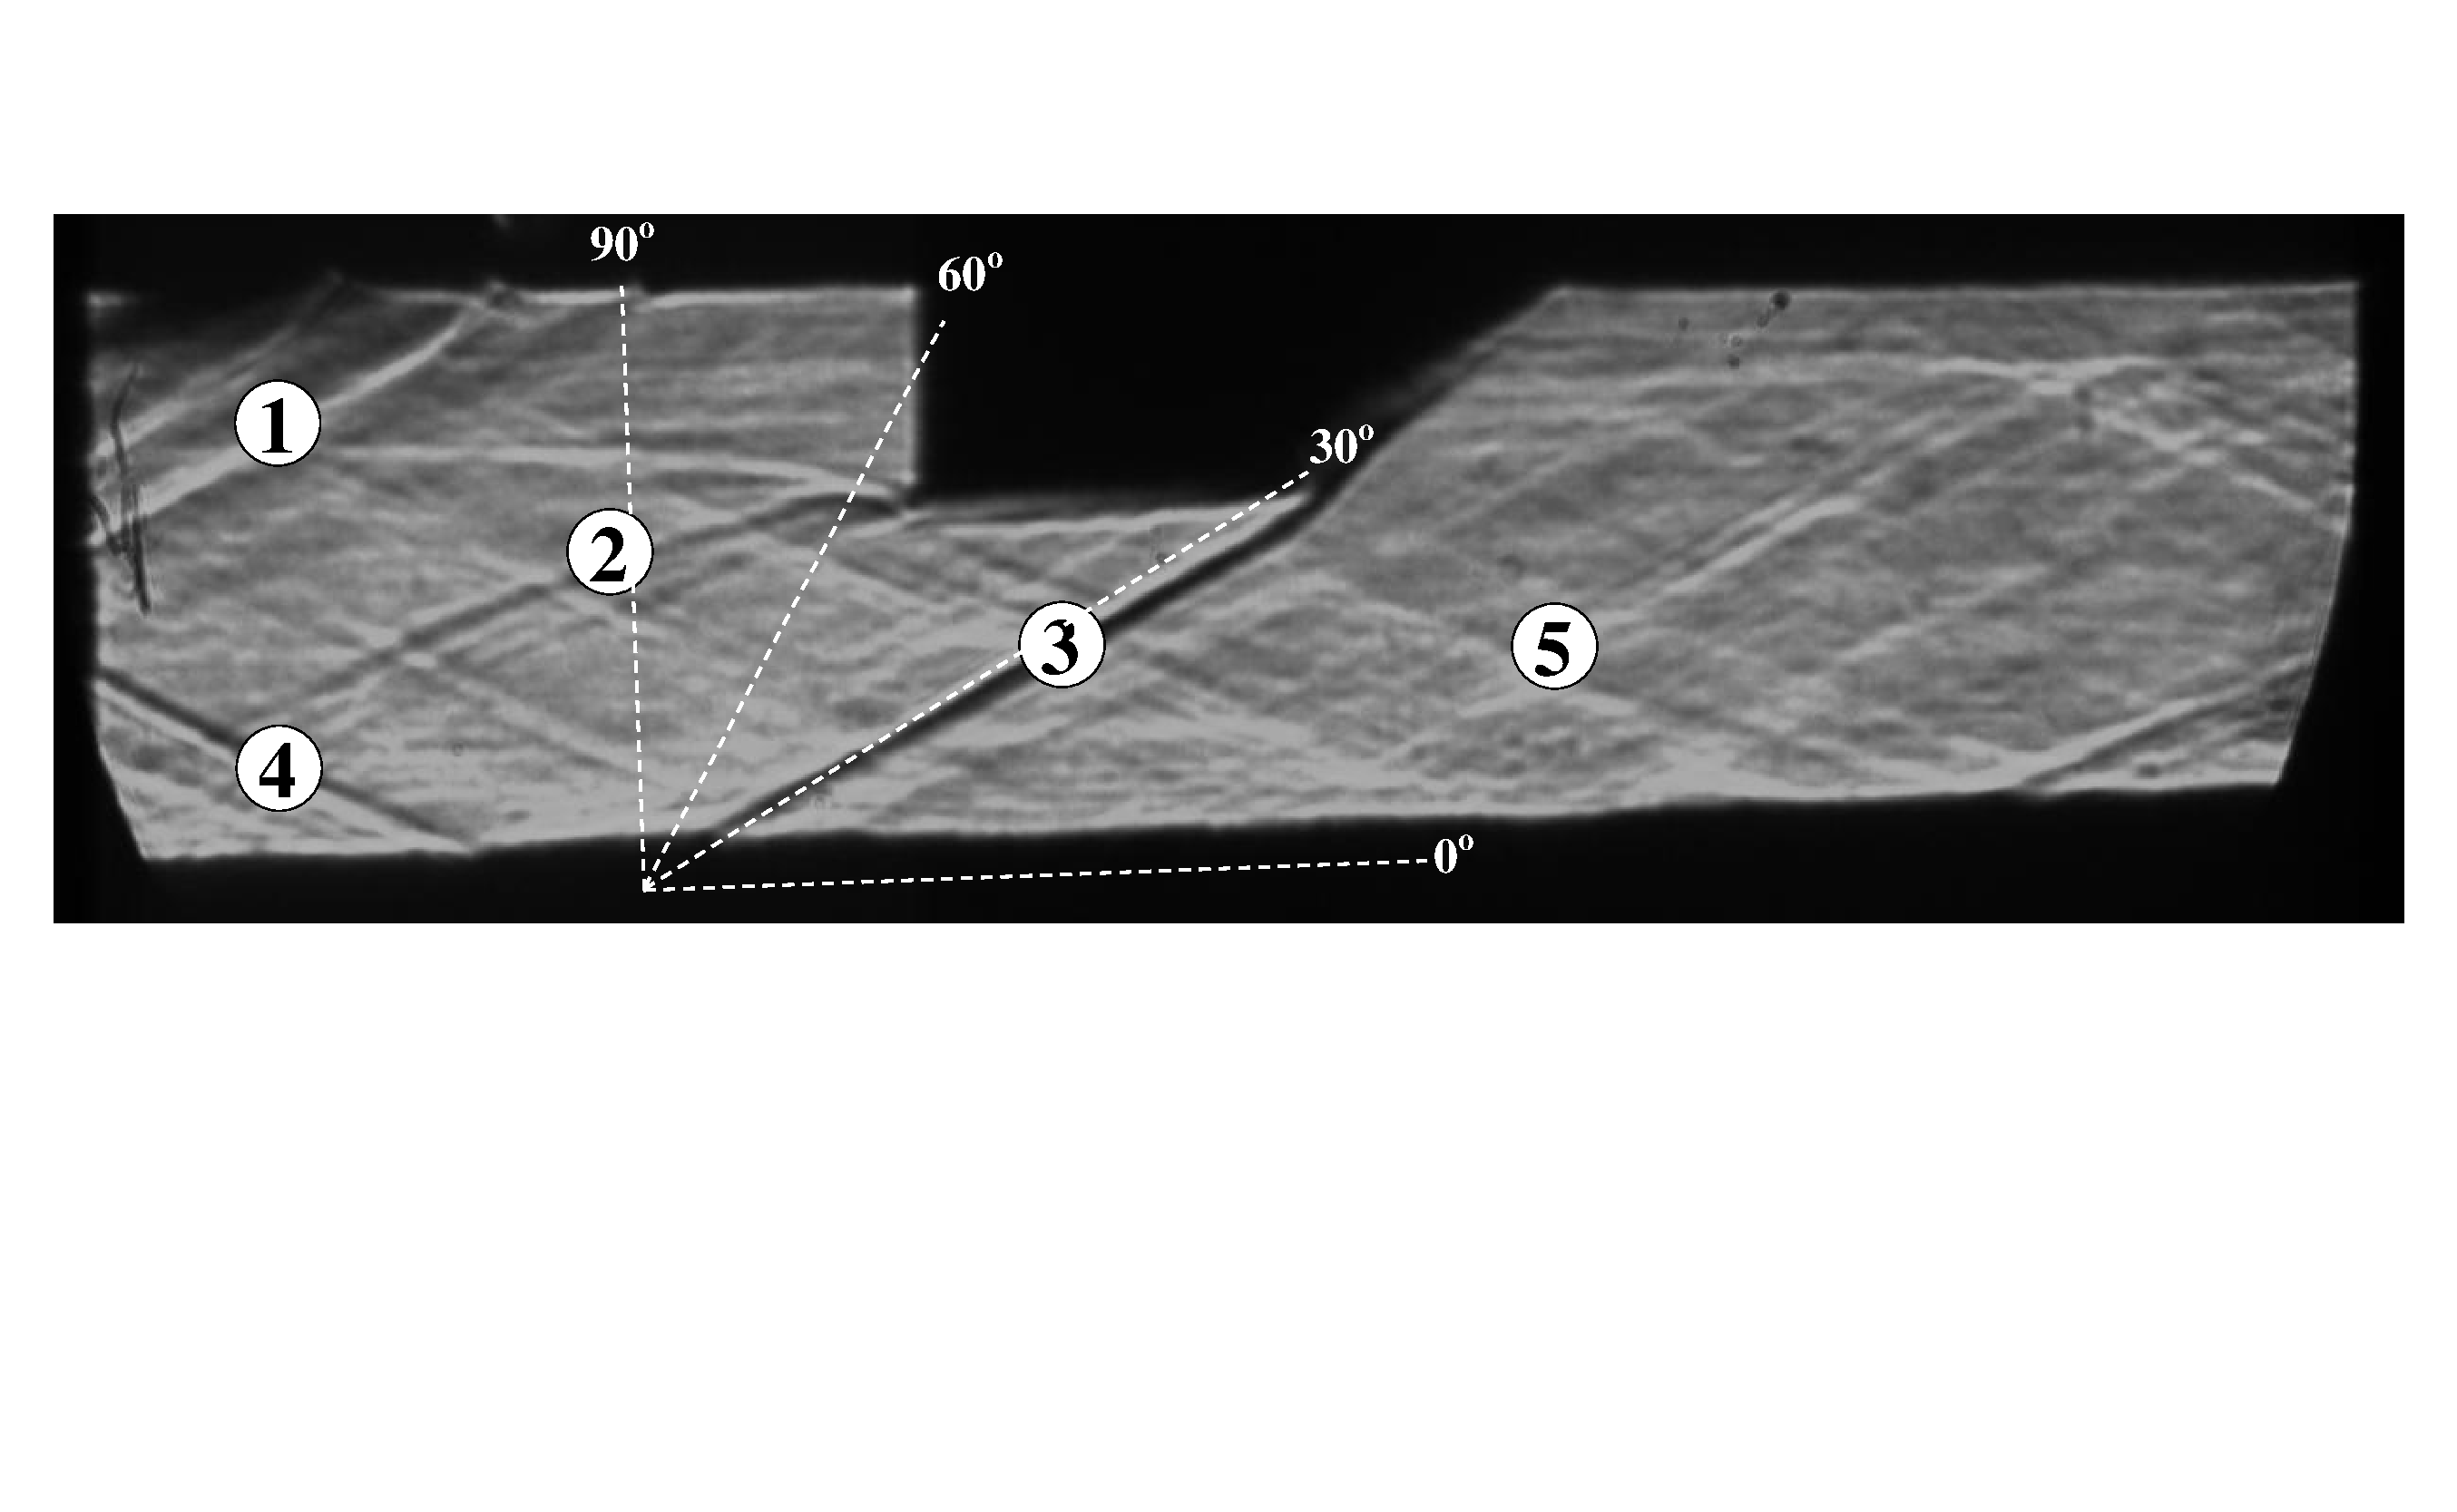
\includegraphics[width=0.95\textwidth]{WaveShadowMarker.pdf}}
\end{center}

\begin{enumerate}
\item 由于燃烧室内流道内壁有突起造成干扰波.
\item 是膨胀波系.
\item 是一个激波.
\item 是3处的激波在壁面的反射波.
\item 前部的壁面扰动与其在风动内部反射的结果.
\end{enumerate}
}


\frame{\frametitle{马赫数分析}
\begin{center}
\fbox{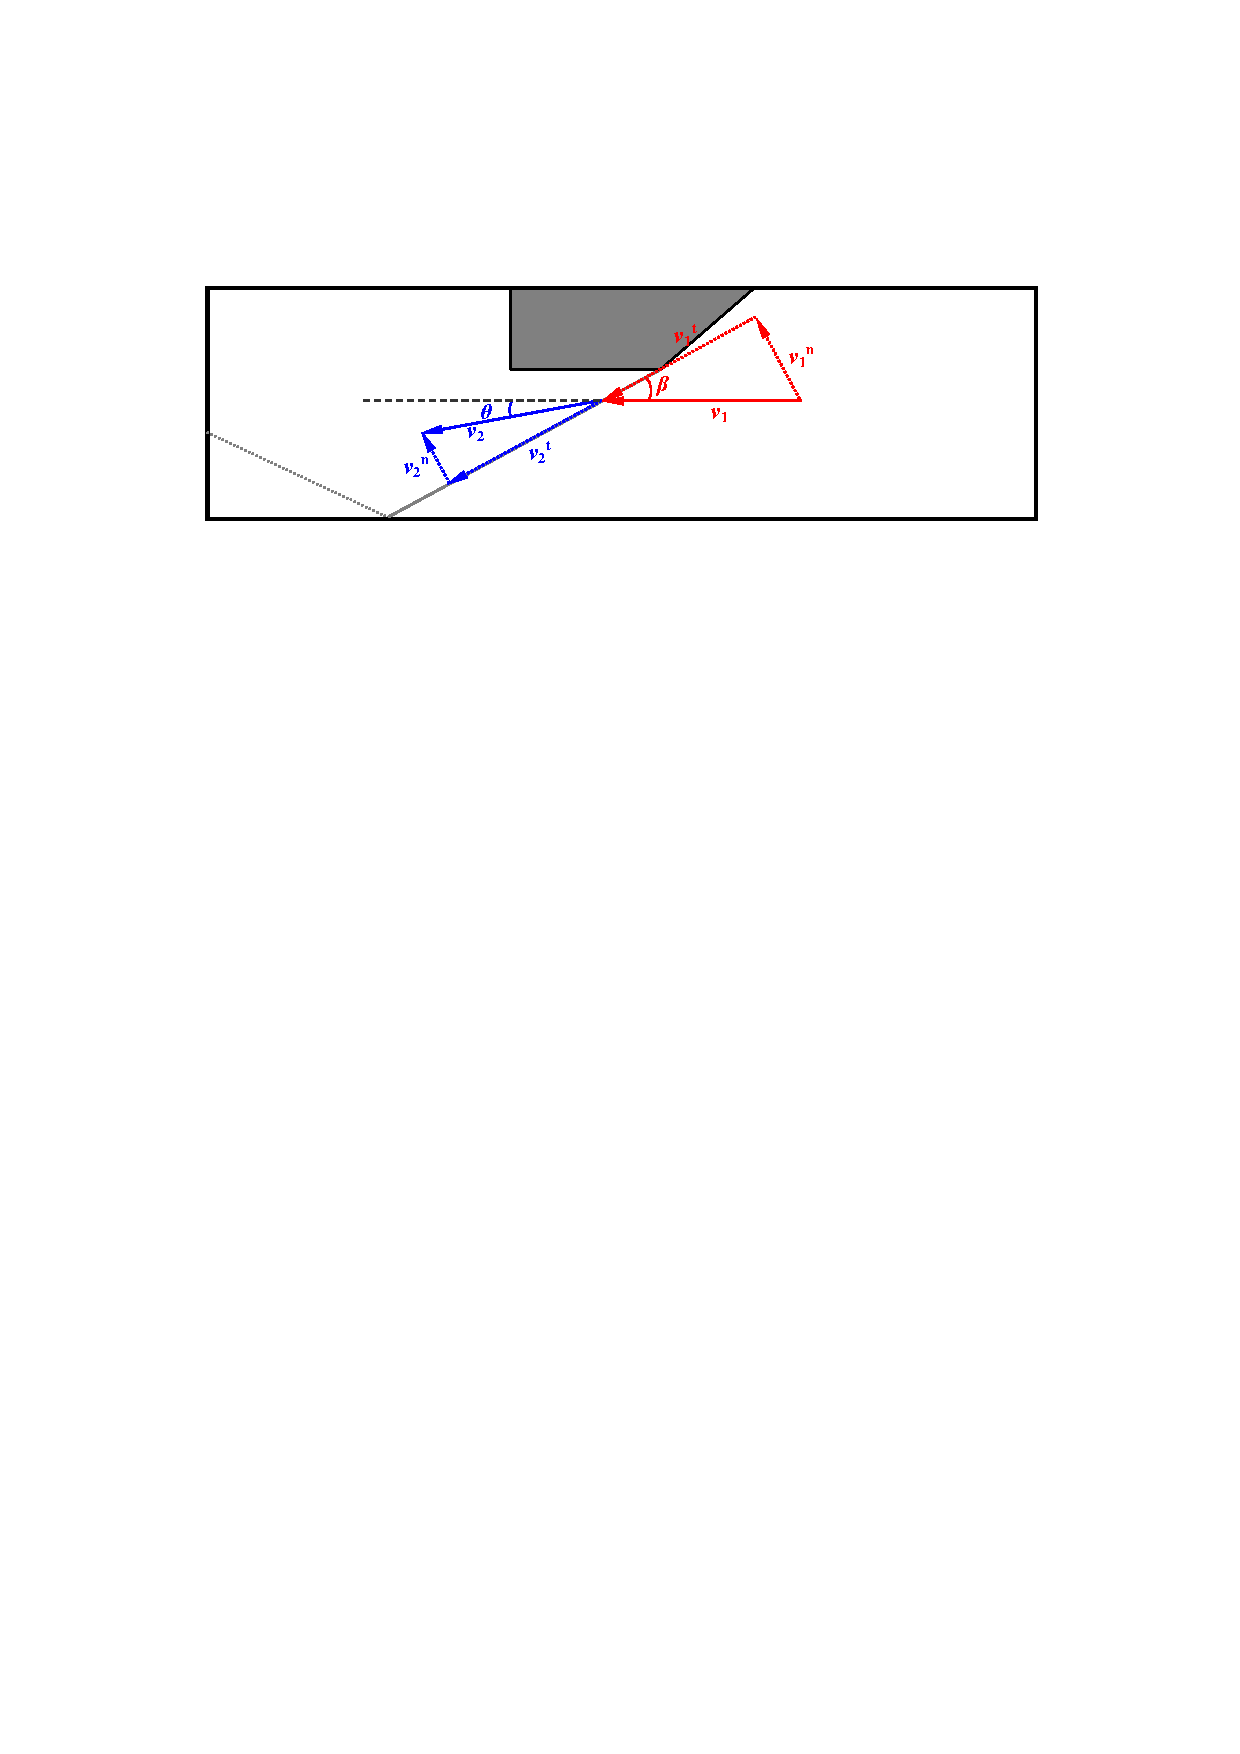
\includegraphics[width=0.95\textwidth]{analysis.pdf}}
\end{center}

{\footnotesize
\[
\tan\beta = v_1^n/v_1^t, \,\,\,\,\,\, \tan(\beta-\theta)=v_2^n/v_1^t, \,\,\,\,\,\, v_1^t = v_2^t
\]
\[
\frac{\tan(\beta-\theta)}{\tan\beta} = \frac{v_2^n}{v_1^n} = \frac{\rho_1}{\rho_2} = \frac{2+(\gamma-1)M_1\sin^2\beta}{(\gamma+1)M_1\sin^2\beta}
\Rightarrow
\tan\theta = \frac{M_1^2\sin^2\beta-1}{M_1^2(\gamma+\cos 2\beta)+2}
\]}
波前波后的速度都应平行壁面, 即$\theta = 0$. 因此$\beta=\pi/2$或$\sin\beta=\frac{1}{M_1}$, 此处应为$\sin\beta=\frac{1}{M_1}$. 可知$\beta\approx\pi/6$, 因此波前马赫数$M_1\approx2$.
}


%\section<presentation>*{参考文献}

\frame{
  \transdissolve
  \frametitle<presentation>{参考文献}

  \beamertemplatebookbibitems
  \begin{thebibliography}{10}

    \bibitem{TeX}
    束继祖, 李华煌. 流场显示技术在流体力学中
的应用和展望. 
    \newblock {力学进展, 1979(01): 002}.

\bibitem{TeX}
    Werle, H. 
    \newblock {Annual Rev. of Fluid Mechanics, 5(1973), 361.}.
    
    \bibitem{TeX}
   李桂春. 风洞试验光学测量方法. 
    \newblock {国防工业出版社, 2008. }.
    
    
 
  \beamertemplatearticlebibitems
  \bibitem{userguide}
Physical solutions of everyday problems in aquatic sciences
    \newblock {\em http://misclab.umeoce.maine.edu/boss/classes/SMS\_491\_2003 /Week\_5.htm}.
    
  \end{thebibliography}
} 

\plainframe{
    \begin{centering}
      \Huge Thank You!!!\par
    \end{centering}
  } 

\end{document}
